\documentclass[conference]{IEEEtran}
\usepackage{amsmath, amssymb, xcolor, graphicx, comment, algorithm, algpseudocode}
\usepackage{soul}
\DeclareMathOperator*{\argmax}{arg\,max}
\DeclareMathOperator*{\argmin}{arg\,min}
\DeclareMathOperator*{\sign}{\mbox{sign}}

\newcommand{\one}{\mathbf{1}}

\usepackage{hyperref} 

\title{Distributed Risk-Aware Bidding Strategy for Incorporating Renewable Generation into Real-Time Electricity Market}
\author{\IEEEauthorblockN{Tommy Truong, Zhihua Qu, and Marwan A. Simaan}
\IEEEauthorblockA{University of Central Florida}}

\begin{document}

\maketitle

\begin{abstract}
This paper proposes a risk-aware optimization framework in which firms' sensitivity to uncertainty serves as a tunable coordination variable. We show that, for a class of stochastic market games, there exists a structured relationship between firms' risk parameters and the resulting Nash equilibrium, such that appropriately chosen risk sensitivities induce Nash equilibria that lie on the Pareto frontier. Based on this insight, we develop a distributed algorithm that allows firms to estimate required aggregate quantities and adapt their risk parameters using only local communication and minimal information exchange. The proposed approach preserves the decentralized nature of the market: firms remain self-interested in their primary decisions, resulting in Pareto-optimal Nash equilibria, and convergence of the distributed algorithm follows from consensus theory under mild connectivity conditions.
\end{abstract}

%\begin{keywords}
{\it Keywords:} Risk-aware bidding, Nash equilibrium, Pareto efficiency, stochastic market,; distributed optimization, renewable energy 
%\end{keywords}

\section{Introduction}

Competitive electricity markets operating under uncertainty exhibit a fundamental tension between individual rationality and collective efficiency.
Renewable energy operators in particular face this challenge acutely: their generation is stochastic and correlated through shared weather conditions,
their output forecasts are uncertain, and their bidding decisions must be submitted before real-time prices are known
\cite{dvorkin2020chance, wong2007pricing, mieth2020distribution}.
When each operator optimizes its own expected profit independently, the resulting Nash equilibrium generally fails to achieve socially optimal outcomes,
even when all firms behave rationally \cite{zhang2016competition, lee2015rational}.
This gap between Nash and Pareto-optimal performance is not merely a theoretical artifact---in markets with many correlated renewable operators,
it translates directly into foregone collective profit and inefficient price signals \cite{asplund2002risk, wambach1999bertrand}.

Existing studies on stochastic Cournot and oligopoly games have examined the impact of uncertainty and risk preferences on equilibrium outcomes,
but typically treat risk attitudes as fixed exogenous parameters \cite{cheng2002bertrand, sakai1989risk, gulpinar2014analysis}.
Under this assumption, the equilibrium is determined once risk preferences are assigned, leaving no room to steer outcomes.
Separately, Pareto efficiency has been studied through centralized optimization or cooperative formulations that require full information sharing
\cite{hobbs2001individual, zhao2010social, su2018integrated}.
These approaches are impractical in deregulated markets where operators are self-interested and unwilling to disclose private cost and forecast data.
The key question that remains unaddressed is whether Nash equilibrium behavior can be reconciled with Pareto-optimal outcomes
\emph{without} centralized coordination or private information disclosure.

This paper answers that question affirmatively by identifying risk sensitivity itself as the coordination variable.
We show that, for a class of stochastic renewable energy market games, there exists a structured relationship between the operators'
risk parameters and the resulting Nash equilibrium bidding strategies, such that appropriately chosen risk levels induce Nash equilibria
that lie on the Pareto frontier.
In this sense, risk is not merely a preference parameter but a mechanism through which self-interested agents can be guided
toward efficient collective outcomes without violating incentive compatibility.

The key enabler for a distributed implementation is that the Pareto condition depends only on the \emph{aggregate} risk level
across operators, not on individual bidding strategies directly.
This means coordination reduces to reaching consensus on a single scalar quantity,
which can be accomplished through local communication without revealing private information.
Building on this insight, we develop a distributed consensus-based algorithm that allows each operator to estimate the required
aggregate quantities and set its risk parameter using only neighborhood communication \cite{molzahn2017survey, yang2019survey}.
Analytical results establish existence and explicit characterization of Pareto-optimal Nash equilibria,
and convergence of the distributed algorithm is established under a mild connectivity condition.
A numerical example illustrates how risk-aware adaptation shifts equilibrium behavior from inefficient Nash outcomes to Pareto-optimal payoffs,
and a sensitivity analysis quantifies the performance impact of physical bid constraints.

The remainder of the paper is organized as follows.
Section~II formulates the stochastic market model and risk-aware objectives.
Section~III characterizes the Nash equilibrium under fixed risk parameters.
Section~IV establishes conditions under which Nash equilibria achieve Pareto efficiency through structured risk allocation.
Section~V presents a distributed algorithm based on consensus to realize these outcomes.
Numerical results are provided in Section~VI, followed by concluding remarks in Section~VII.

\section{Problem Formulation}

In this paper, we consider the simple case that all traditional generation assets are owned by a single utility company\footnote{The proposed results apply to the general case of multiple utility companies of individual cost functions except for notational complexity.} while renewable generation are operated by individual entities (one of which could be the utility company). And, the utility company and the renewable generation operators are the participants in both day-ahead and real-time electricity markets for profit. 

In an electricity market, utility aims to optimize a composite objective function in the form of 
\begin{equation} 
J(P_g) = a_2 P_g^2 + a_1 P_g + a_0, \label{eq:Jm}
\end{equation}
where $a_i$ are cost coefficients, and $P_g$ is the aggregated power of traditional generation. For simplicity, marginal costs of operating renewables and battery storage sites are modeled as zero, and hence they need not to be included explicitly in objective function \eqref{eq:Jm}. 

Let $\Omega$ be the set of renewable generation operators, with $n=|\Omega|$ being its cardinal. For the day-ahead market, their renewable generations, $P_j$ for $j\in\Omega$, are modeled as stochastic variables, and similarly the grid total load $P_L$ is also modeled as a stochastic variable. Lets form the whole vector of random variables as 
\begin{equation} 
x = \begin{bmatrix} P_1 & \cdots & P_n & P_L \end{bmatrix}^T.  \label{eq:x}
\end{equation}
We assume that probability distribution of random vector $x$ is Gaussian as follows:
\[ f(x) = (2\pi)^{-\frac{n+1}{2}}\Sigma^{-\frac{1}{2}} e^{-\frac{1}{2}(x-x^o)^T\Sigma^{-1}(x-x^o)},  \]
where  $x^o=\mathbb{E}[x]$ is the vector of forecast (for the day-ahead market), and 
\begin{eqnarray*}
\Sigma & = & \mathbb{E}[(x-x^o)(x-x^o)^T] \\
& = & \begin{bmatrix} \sigma_{11} & \cdots & \sigma_{1n} & \sigma_{1L} \\ \vdots & \cdots & \vdots & \vdots \\ \sigma_{n1} & \cdots & \sigma_{nn} & \sigma_{nL} \\ \sigma_{1L} & \cdots & \sigma_{nL} & \sigma_{LL}
\end{bmatrix},  
\end{eqnarray*}
is the covariance matrix with $\sigma_{ij}=\sigma_{ji}$. In the covariance matrix, the last row and column correspond to covariances between the renewable generations and the load while $\sigma_{LL}=\sigma_L^2>0$ is the variance of the load. It is known that 
$\sigma_{ii}=\sigma_i^2>0$, $\sigma_{ij}=\rho_{ij}\sigma_i\sigma_j$, $\sigma_{iL}=\rho_{iL}\sigma_i\sigma_L$, where $\rho_{ij},\rho_{iL}\in[0,1]$. Typically, $\rho_{ij},\rho_{iL}\not=0$ because renewable generations and load are correlated through the projected weather condition. 

The day ahead market clears the projected aggregated power generation $P_g^o$ and its associated price $\lambda^o$ by minimizing $J(P_g^o)$ under the following power balance constraint:
\begin{equation} 
P_g^o + \sum_{j=1}^n \alpha_j x_j^o  = x_{n+1}^o, \label{eq:DA_power}
\end{equation}
where $x_{n+1}^o=P_L^o$, $\alpha_j\in[0,1]$ if no overbidding is allowed or $\alpha_j\in[0,\infty)$ if overbidding is permitted, and $\alpha_j x_j^o =\alpha_j P_j^o$ represent the bids by the renewable generation operators into the day-ahead market. Similarly, the real-time market clears the aggregated power generation $P_g$ and its associated price $\lambda$ by minimizing $J(P_g)$ under the following real-time power balance constraint:
\begin{equation} 
P_g + \sum_{j=1}^n x_j   = x_{n+1}. \label{eq:RT_power}
\end{equation}
It is well known that, with global information, day-ahead price $\lambda^o$ and real-time $\lambda$ are the dual variables associated with constraints \eqref{eq:DA_power} and \eqref{eq:RT_power}, respectively. 

The renewable generation operators aim to maximize the following objectives\footnote{Strictly speaking, we should use $J_i^{\prime} = \Pi_i - \beta_i \mathbb{E}[(\Pi_i - \mathbb{E}[\Pi_i])^2]$ which also yields a second-order polynomial in $\alpha_i$ as does \eqref{eq:J_i} but involves calculations of higher moments. Accordingly, \eqref{eq:J_i} is adopted instead.} individually:
\begin{subequations}
\begin{equation} 
J_i = \Pi_i - \beta_i \mathbb{E}[(\lambda - \lambda^o)^2], \label{eq:J_i}
\end{equation}
where $\beta_i\in\mathbb{R}$, 
\begin{equation} 
\Pi_i %= \lambda^o \alpha_i P_i^o + \mathbb{E}[\lambda (P_i - \alpha_i P_i^o)] 
= \lambda^o \alpha_i x_i^o + \mathbb{E}[\lambda (x_i - \alpha_i x_i^o)], \label{eq:Pi_i}
\end{equation}
\end{subequations}
and the pair $\{\alpha_i, \; \beta_i\}$ represents the bidding strategy of the $i$-th operator into the electricity markets. If $\beta_i=0$ is chosen, the $i$-th entity aims to maximize its average profit from the total revenues from participating in the day ahead and real time markets. By selecting $\beta_i>0$, the $i$-th entity also attempts to reduce its profit variation by suppressing variations of real time price $\lambda$ around day ahead price $\lambda^o$.  By choosing $\beta_i<0$, the $i$th entity tries to maximize its profit by encouraging more variations of real time price $\lambda$ around day ahead price $\lambda^o$. In other words, the $i$-th entity is risk averse if $\beta_i>0$ and risk seeking if $\beta_i<0$.

The objective of this paper is to show the following advantages by introducing the risk aware bidding strategy of $\{\alpha_i, \; \beta_i\}$: (i) achieving Pareto-optimal Nash equilibria that maximize the total profit $\sum_{i=1}^n \Pi_i$; 
% (equivalently, maximizing $g(\alpha_1^*,\ldots,\alpha_n^*)$ as defined in \eqref{eq:G});
(ii) enabling distributed implementation without centralized coordination; (iii) maintaining incentive compatibility as firms remain self-interested; and (iv) preserving privacy through minimal information exchange. Power grid congestion is not considered in the paper but can be considered.

\section{Centralized Risk-Aware Solution Under Global Information}

The electricity markets are bi-level optimization problems linked together by dual variables. At the upper level, they are quadratic optimization problems with equality constraints, that is, the markets perform their economic dispatch with the following Lagrangians: 
\begin{subequations}
\begin{equation} 
L^o = a_2(P_g^o)^2+a_1P_g^o+a_0 + \lambda^o\left(x_{n+1}^o- P_g^o-\sum_{j=1}^n \alpha_j x_j^o \right), \label{eq:L*}
\end{equation}
\begin{equation} 
L = a_2P_g^2+a_1P_g+a_0 + \lambda^o\left(x_{n+1}-P_g-\sum_{j=1}^n x_j\right). \label{eq:L}
\end{equation}
\end{subequations}
Applying the first-order optimality condition to the Lagrangians yields the following solutions for the prices:
\begin{subequations}
\begin{equation} 
\lambda^o = 2a_2P_g^o +a_1 = 2a_2\left(x_{n+1}^o-\sum_{j=1}^n \alpha_j x_j^o \right) +a_1 , \label{eq:lambda*}
\end{equation}
\begin{equation} 
\lambda = 2a_2P_g+a_1=2a_2\left(x_{n+1}-\sum_{j=1}^n x_j \right) + a_1. \label{eq:lambda}
\end{equation}
\end{subequations}

The lower level optimization problems are also quadratic, and the centralized solutions under global information are summarized into the following lemma and theorem. Lemma 1 provides the solution of cooperative optimization when all the entities bind themselves together and act as one. In this case, the best outcome for the group is achieved under the risk neutral strategy.

\noindent {\bf Lemma 1:} {\it Consider the case that all renewable generation entities form a coalition by sharing all the information and setting $\alpha_i=\alpha$ and $\beta_i=\frac{1}{n}\beta$, respectively. Then, for any choice of $\beta\in[-(4a_2)^{-1},\; +\infty)$, the optimal bidding strategy to optimize objective function $\sum_i J_i$ with $J_i$ in \eqref{eq:J_i} is
\begin{equation}
\alpha^* = \frac{1 + 4a_2 \beta}{2(1 + 2a_2\beta)}.
\label{eq:alpha_1}
\end{equation}
In addition, by further choosing $\beta_i$ to optimize $\sum_i \Pi_i$ with $\Pi_i$ in \eqref{eq:Pi_i}, the optimal bidding strategy $\{\alpha^*, \; \beta^*\}$ is given by}
\begin{equation}
\alpha^*  =  \frac{1}{2}, \quad
\beta^*  =  0.
\label{eq:optimal_1}
\end{equation}

\noindent {\bf Proof:} It follows from \eqref{eq:Pi_i} and \eqref{eq:lambda*} that, if $\alpha_i=\alpha$, 
\begin{eqnarray*}
\Pi_r & = & \sum_{j=1}^n \Pi_j = \lambda^o \alpha x_r^o +  \mathbb{E}[\lambda (x_r-\alpha x_r^o)] \\
 \lambda^o   & = & 2a_2\left(x_{n+1}^o-\alpha x_r^o \right) +a_1,
\end{eqnarray*}
where $x_r = \sum_{j=1}^n x_j$ is the total renewable generation, and $x_r^o = \sum_{j=1}^n x_j^o$. Substituting \eqref{eq:lambda} into the above equations yeld
\begin{eqnarray}
\Pi_r & = &  [2a_2\left(x_{n+1}^o-\alpha x_r^o \right) +a_1] \alpha x_r^o \nonumber \\
&& + \mathbb{E}[(2a_2\left(x_{n+1}-x_r \right) + a_1)(x_r-\alpha x_r^o)] \nonumber \\
  & = & 2a_2\alpha(1-\alpha)(x_r^o)^2 +a_1x_r^o  + 2a_2\mathbb{E}[\left(x_{n+1}x_r-x_r^2 \right)] \nonumber\\
   & = & 2a_2\alpha(1-\alpha)(x_r^o)^2 +a_1x_r^o \nonumber \\
   && + 2a_2\left(x_{n+1}^ox_r^o+\sigma_{rL}-(x_r^o)^2-\sigma_r^2 \right), \label{eq:Pi_r_exp}
\end{eqnarray}
where $\one$ is the $n$-dimensional column vector of $1$s and 
\begin{eqnarray*}
    \sigma_r^2 & = & \mathbb{E}[(x_1+\cdots+x_n-(x_1^o+\cdots+x_n^o))^2] \\
    & = & \mathbb{E}[ \one^T (x-x^o)(x-x^o)^T\one] \\
    & = & \one^T \Sigma \one. 
\end{eqnarray*}
On the other hand, it follows from \eqref{eq:J_i}, \eqref{eq:lambda*}, and \eqref{eq:lambda} that, if $\beta_i = \frac{1}{n}\beta$,
\begin{eqnarray*}
J_r & = & \sum_{j\in\Omega} J_j \\
 & = & \Pi_r  - \beta \mathbb{E}[2a_2 (x_{n+1}-x_{n+1}^o -x_r +\alpha x_r^o)^2] \\
 & = & 2a_2\alpha(1-\alpha)(x_r^o)^2  - 4a_2^2  \beta  (1-\alpha)^2 (x_r^o)^2 \\
 & & +a_1x_r^o + 2a_2\left(x_{n+1}^ox_r^o+\sigma_{rL}-(x_r^o)^2-\sigma_r^2 \right)\\
 && - 4a_2^2  \beta (\sigma_L^2+\sigma_r^2 - 2\sigma_{rL}). 
\end{eqnarray*}
Using the above expression, taking the partial derivative of $J_r$ with respect to $\alpha$, and setting the partial derivative to zero yield optimal bidding strategy \eqref{eq:alpha_1}. 

Substituting solution \eqref{eq:alpha_1} into 
\eqref{eq:Pi_r_exp} and taking the partial of $\Pi_r$ with respect to $\beta$ result in
\[ \frac{\partial \Pi_r}{\partial \beta} = - 2a_2(x_r^o)^2\frac{4a_2^2\beta}{(1+2a_2\beta)^3}, \]
which yields the optimal bidding strategy \eqref{eq:optimal_1}. This completes the proof. \hfill $\Box$

It follows from \eqref{eq:alpha_1} that
\[ \lim_{\beta\rightarrow-1/(4a_2)} \alpha = 0, \quad  \lim_{\beta\rightarrow0} \alpha = 0.5, \quad \lim_{\beta\rightarrow +\infty} \alpha = 1. \]
Since $\alpha\in[0,1]$, the design parameter $\beta$ translates an operator's risk tolerance level into a specific choice of $\alpha$ value. Although the values correspond to risk neutral choices may change, this translation is applicable to not only cooperative coalition game but also noncooperative games. 

The following theorem provides the solution to non-cooperative optimization in which each agent devises its strategy according to its own objective function $J_i$. 

\noindent {\bf Theorem 1:} {\it For renewable energy generation operators, their oligopoly game always has a Nash equilibrium. Specifically,
for any choice of $\beta_i\in[-(4a_2)^{-1},+\infty)$, the optimal bidding strategy $\alpha_i^*$ to optimize objective $J_i$ in \eqref{eq:J_i} forms a Nash equilibrium corresponding to the solution to the linear algebraic equation:
denoting $\boldsymbol{\alpha}^*=[\alpha_1^* \; \cdots \; \alpha_n^*]^T$,
\begin{equation}
A \boldsymbol{\alpha}^* = B,
\label{eq:alpha_i}
\end{equation}
where $x_r^o = \sum_{j=1}^n x_j^o$, $\eta_i = x_i^o/x_r^o\geq0$ with $\sum_{i=1}^n \eta_i=1$, and
\[ A=[A_{ij}], \quad A_{ij} = \left\{ \begin{array}{ll} 2(1+2a_2\beta_i)\eta_i & \mbox{if $i=j$} \\
(1+4a_2\beta_i)\eta_j & \mbox{if $i\not=j$}\end{array} \right., \]
and
\[ B=[B_i], \quad B_i = (1+4a_2\beta_i). \]
In addition,  the total profit $\Pi=\sum_{i=1}^n\Pi_i$ can be maximized by choosing $\beta_j$ to maximize the following function: 
\begin{equation} 
g(\boldsymbol{\alpha}^*) = f(\boldsymbol{\alpha}^*) \left[ 1 - f(\boldsymbol{\alpha}^*)  \right](x_r^o)^2,
\label{eq:G}
\end{equation} 
where  
\begin{equation} 
f(\boldsymbol{\alpha}) \stackrel{\triangle}{=} \sum_{i=1}^n  \alpha_i \eta_i.  
\label{eq:F}
\end{equation} 
}

\noindent {\bf Proof:} It follows from \eqref{eq:Pi_i},  \eqref{eq:lambda*}, and \eqref{eq:lambda} that 
\begin{eqnarray}
\Pi_i & = & \left[ 2a_2\left(x_{n+1}^o-\sum_{j=1}^n \alpha_j x_j^o 
  \right) +a_1 \right] \alpha_i x_i^o \nonumber \\ && 
  + \mathbb{E}\left[\left(2a_2\left(x_{n+1}-\sum_{j=1}^n x_j \right) + a_1\right) (x_i - \alpha_i x_i^o)\right] \nonumber \\
  & = & 2a_2\sum_{j=1}^n\alpha_i(1-\alpha_j)x_j^o x_i^o +a_1 x_i^o  \nonumber \\ 
  && + 2a_2\mathbb{E}\left[\left(x_{n+1}-\sum_{j=1}^n x_j \right) x_i\right] \nonumber\\
   & = & 2a_2\sum_{j=1}^n\alpha_i(1-\alpha_j)x_j^o x_i^o +a_1 x_i^o  \nonumber \\ 
  && + 2a_2\left(x_{n+1}^o x_i^o + \sigma_{iL}- \sum_{j=1}^n (x_j^o  x_i^o+ \sigma_{ij})\right), \label{eq:Pi_j_exp}
\end{eqnarray}
where the identity $\mathbb{E}[x_ix_j]=x_i^ox_j^o+\sigma_{ij}$ is used. On the other hand, It follows from \eqref{eq:lambda*} and \eqref{eq:lambda} that 
\begin{eqnarray} 
&& \mathbb{E}[(\lambda - \lambda^o)^2] \nonumber \\
& = & 
4a_2^2  \mathbb{E}\left[\left(x_{n+1}-x_{n+1}^0 +\sum_{j=1}^n x_j-\alpha_j x_j^o\right)^2\right] \nonumber \\
& = & 4a_2^2\left[\sigma_{LL} + 2\sum_{j=1}^n \sigma_{jL} + 2 \sum_{j=1}^n \sum_{l=1}^n \sigma_{jl} \right. \nonumber \\
&& \left.+ \left(\sum_{j=1}^n (1-\alpha_j) x_j^o\right)^2 \right]
, \label{eq:sigma_lambda}
\end{eqnarray}
The expression of $J_i$ defined in \eqref{eq:J_i} becomes explicit in terms of $\alpha_i$ by combining \eqref{eq:Pi_j_exp} and \eqref{eq:sigma_lambda}. Taking the partial derivatives of $J_i$ with respect to $\alpha_i$ yields
\begin{subequations}
\begin{eqnarray} 
\frac{\partial J_i}{\partial \alpha_i} & = &  2a_2(1+4a_2\beta_i) \sum_{j=1}^n(1-\alpha_j)x_j^o x_i^o \nonumber \\&& 
- 2a_2 \alpha_i (x_i^o)^2, \label{eq:p1_Ji} \\
\frac{\partial J^2_i}{\partial \alpha_i^2} & = & - 4a_2(1+2a_2\beta_i) (x_i^o)^2 <0 \;\;\; \forall \beta_i\geq-\frac{1}{4a_2}. \hspace*{.3in} \label{eq:p2_Ji}
\end{eqnarray}
\end{subequations}
Inequality \eqref{eq:p2_Ji} shows that Nash equilibrium exists, and setting \eqref{eq:p1_Ji} to be zero yields 
\begin{equation}
   (1+4a_2\beta_i) \sum_{j=1}^n(1-\alpha_j)x_j^o 
- \alpha_i x_i^o=0, \label{eq:p1Ji=0}
\end{equation}  
which yields matrix equation \eqref{eq:alpha_i} to solve for Nash equilibrium. 

It follows from \eqref{eq:alpha_i} that $\alpha_i^*$ are functions of $\beta_j$. We know from  \eqref{eq:Pi_j_exp} that 
\begin{eqnarray}
    \Pi & = & \sum_i \Pi_i \nonumber \\
     & = & 2a_2\left[ g(\boldsymbol{\alpha}) - \left(x_r^o\right)^2 + x_{n+1}^o x_r^o\right]  +a_1 x_r^o  \nonumber \\ 
     && + 2a_2 \left[ \sum_{i=1}^n \sigma_{iL} -\sum_{i=1}^n\sum_{j=1}^n\sigma_{ij}\right], \label{eq:Pi_exp}
\end{eqnarray}
where
\[ g(\boldsymbol{\alpha}) \stackrel{\triangle}{=} \sum_{i=1}^n  \alpha_i x_i^o  \sum_{j=1}^n (1-\alpha_j ) x_j^o. \]
Hence, $\Pi$ is maximized if function $g(\cdot)$ is maximized by choosing $\beta_j$.
Simplifying the above expression of $g(\cdot)$ yields \eqref{eq:G}. This completes the proof. \hfill $\Box$

Theorem 1 extends the results in \cite{Chow2017} in several ways. First, load uncertainties and correlations among the renewable generations are considered.  As a result, we know from \eqref{eq:Pi_exp} that the degradation of total profit function $\Pi$ due to uncertainties is 
\[ \Delta \Pi = 2a_2 \left[ \sum_{i=1}^n\sum_{j=1}^n\sigma_{ij}- \sum_{i=1}^n \sigma_{iL}\right], \]
is less as long as there is some correlation (e.g., due to weather) between renewable generation and load variation. Second, risk aware bidding strategies are considered, specifically, theorem 1 allows us to study and compare three classes of bidding strategies: risk neutral, risk adverse, and risk seeking. The latter two correspond to optimization of design parameters $\beta_j$. 

Theorem 1 shows that the Nash equilibrium in terms of design parameters $\beta_j$ can be further optimized, and the optimal choices of $\beta_j$ are the main subject of this paper. To illustrate some of the specifics, lets first consider the two simple cases: $n=1$ and $n=2$. And the corresponding results are provided by the subsequent corollaries, followed by the risk neutral strategy for the general case of $n$ operators. 

\noindent  {\bf Corollary 1:} {\it If $n=1$, the optimal coalition (C) biding strategy becomes the same as that in lemma 1 and with $g^C(\alpha^*)=\frac{1}{4} (x_r^o)^2$.}

\noindent  {\bf Corollary 2:} {\it In the case of duopoly ($n=2$), the Nash bidding strategies with respect to $J_i$ are:
\begin{subequations}
\label{eq:2p-alpha}
\begin{equation}
\alpha_1^*= \frac{(1+4a_2\beta_1)}{3+4a_2(\beta_1+\beta_2)}\eta_1^{-1}, 
\label{eq:2p-alpha1}
\end{equation} 
\begin{equation}
 \alpha_2^*= \frac{(1+4a_2\beta_2)}{3+4a_2(\beta_1+\beta_2)}\eta_2^{-1}, \, 
\label{eq:2p-alpha2}
\end{equation} 
\end{subequations}
Furthermore, $\beta_i$ can be optimized with respect to $(\Pi_1+\Pi_2)$, and the outcomes are strategically dependent as follows. 
\begin{itemize}
\item Risk neutral (RN) optimal bidding strategy is $\beta_i^{NR}=0$ for $i=1,2$; and the corresponding optimized profit is:
\begin{equation}
g^{RN}(\alpha_1^*, \alpha_2^*)  =  \frac{2}{9}(x_r^o)^2. 
\label{eq:2p-neutral}
\end{equation} 
\item Risk seeking (RS) optimal bidding strategy  and the corresponding enhanced optimal profit are:
\begin{subequations}
\label{eq:2p-RS}
\begin{equation}
\beta_1^{RS}+\beta_2^{RS}=-\frac{1}{4a_2},
\label{eq:2p-RS-beta}
\end{equation} 
\begin{equation}
g^{RS}(\alpha_1^*,\alpha_2^*) = \frac{1}{4}(x_r^o)^2 = g^C(\alpha^*)   > g^{RN}(\alpha_1^*, \alpha_2^*). 
\label{eq:2p-RS-g}
\end{equation} 
\end{subequations}
\end{itemize} }

 \noindent {\bf Proof:} It follows from \eqref{eq:alpha_i} that 
 \begin{eqnarray*}
  && \begin{bmatrix} 2(1+2a_2 \beta_1)\eta_1 & (1+4a_2\beta_1)\eta_2  \\ (1+4a_2\beta_2)\eta_1  & 2(1+2a_2 \beta_2)\eta_2  \end{bmatrix}   
  \begin{bmatrix}  \alpha_1^* \\ \alpha_2^* \end{bmatrix}  \\
  & = &  \begin{bmatrix}  (1+4a_2\beta_1) \\ (1+4a_2\beta_2)\end{bmatrix},
      \end{eqnarray*}
 whose solution is given by \eqref{eq:2p-alpha}.

It follows from \eqref{eq:2p-alpha} that, when $\beta_i=0$,
\[ \alpha_1^* = \frac{1}{3}\eta_1^{-1}, \quad \alpha_2^* = \frac{1}{3}\eta_2^{-1}. \]
Substituting the above solutions into \eqref{eq:F} and \eqref{eq:G} yields \eqref{eq:2p-neutral}.

To further optimize the risk-aware bidding strategy \eqref{eq:2p-alpha}, we rewrite the solution as
\[ \alpha_1^* = \theta_1 \eta_1^{-1}, \quad \alpha_2^* = \theta_2\eta_2^{-1}, \]
where 
\begin{equation}
    \theta_i = \frac{(1+4a_2\beta_i)}{3+4a_2(\beta_1+\beta_2)}. \label{eq:theta}
\end{equation} 
It follows from \eqref{eq:F} and \eqref{eq:G} that 
\begin{eqnarray*}
    g(\alpha_1^*, \alpha_2^*) & = & (\theta_1+\theta_2) [1- (\theta_1+\theta_2)] (x_r^o)^2, 
\end{eqnarray*}
which is maximized to be that in \eqref{eq:2p-RS-g} if
\[ \theta_1+\theta_2=\frac{1}{2}. \]
Invoking \eqref{eq:theta} and solving for the optimal values of $\beta_i$ yields $\beta_i^{RS}$ in \eqref{eq:2p-RS-beta}. This completes the proof. \hfill $\Box$

\noindent  {\bf Corollary 3:} {\it In the general case of $n>2$, the optimal risk-neutral biding strategy is 
\begin{equation}
    \alpha_i^* = \frac{1}{n+1}\eta_i^{-1},\label{eq:alpha_i_0} 
\end{equation} 
and the total profit $\Pi$ in \eqref{eq:Pi_exp} is optimized with 
\[ g^{RN}(\boldsymbol{\alpha}^*)=\frac{n}{(n+1)^2} (x_r^o)^2. \]}

\noindent {\bf Proof:} It follows that, when $\beta_i=0$, the matrix equation \eqref{eq:alpha_i} reduces to 
\[ \left[\mbox{diag}\{\eta_1,\cdots,\eta_n\} + \one \boldsymbol{\eta}^T \right] \boldsymbol{\alpha}=\one, \]
where $\boldsymbol{\eta}=[\eta_1 \; \cdots \; \eta_n]^T$ and $\one=[1 \; \cdots \; 1]^T$. It is simple to verify that the solution is given by \eqref{eq:alpha_i_0}. And, the corresponding total profit can be calculated in terms of \eqref{eq:G} and \eqref{eq:F}.  \hfill $\Box$

In the risk-neutral case ($\beta_i = 0$), the Nash equilibrium is given directly by Corollary~3: $\alpha_i^* = \frac{1}{n+1}\eta_i^{-1}$. Overbidding ($\alpha_i^* > 1$) occurs if and only if $\eta_i < \frac{1}{n+1}$, that is,
\begin{equation}
    \eta_i \geq \frac{1}{n+1} \;\;\; \forall i \label{eq:eta_0}
\end{equation}
is the no-overbidding condition. Physically, $\alpha_i^* > 1$ means operator $i$ commits to deliver more power than its forecast capacity $x_i^o$ into the day-ahead market, exposing itself to real-time shortfall.

When condition~\eqref{eq:eta_0} fails, the no-overbidding policy imposes the box constraint
\begin{equation}
0\le \bar{\alpha}_i \le 1,\qquad
\bar{\alpha}_i = \min\{1,\, \alpha_i^*\}, \label{eq:alpha_clamp}
\end{equation}
but the constrained equilibrium is not obtained by merely projecting the unconstrained profile componentwise. Indeed, from the first-order condition~\eqref{eq:p1Ji=0}, any unsaturated operator must still satisfy
\[
(1+4a_2\beta_i)\sum_{j=1}^n(1-\bar{\alpha}_j)x_j^o-\bar{\alpha}_i x_i^o=0.
\]
For the risk-neutral case $\beta_i=0$, define
\[
t^{RN}\triangleq 1-\bar{f}^{RN},\qquad
\bar{f}^{RN}=\sum_{i=1}^n \eta_i\bar{\alpha}_i .
\]
Then the constrained Nash solution has the closed form
\begin{equation}
\bar{\alpha}_i=
\min\!\left\{1,\;\frac{t^{RN}}{\eta_i}\right\},
\label{eq:alpha_clamp_RN_closed}
\end{equation}
or equivalently
\[
\eta_i\bar{\alpha}_i=\min\{\eta_i,t^{RN}\},\qquad
t^{RN}=1-\sum_{i=1}^n \min\{\eta_i,t^{RN}\}.
\]
Let the shares be ordered as
\[
\eta_{(1)}\le \eta_{(2)}\le \cdots \le \eta_{(n)},
\]
and suppose exactly the first $m$ operators are saturated, i.e.,
$\Omega_s=\{(1),\ldots,(m)\}$. Then
\begin{equation}
t_m^{RN}=
\frac{1-\sum_{k=1}^m \eta_{(k)}}{n-m+1},
\label{eq:tbar_RN}
\end{equation}
and the constrained bids are
\begin{equation}
\bar{\alpha}_{(i)}=
\left\{
\begin{array}{ll}
1, & i\le m,\\[2mm]
\dfrac{1-\sum_{k=1}^m\eta_{(k)}}{(n-m+1)\eta_{(i)}}, & i>m,
\end{array}
\right.
\label{eq:alpha_bar_RN_active}
\end{equation}
where $m$ is the unique index satisfying
\[
\eta_{(m)}\le t_m^{RN}\le \eta_{(m+1)}.
\]
Accordingly, the aggregate bidding fraction for the risk-neutral constrained equilibrium is
\begin{equation}
\bar{f}^{RN}
=
\sum_{i=1}^m\eta_{(i)}
+
\frac{n-m}{n-m+1}
\left(1-\sum_{i=1}^m\eta_{(i)}\right)
=
1-\frac{1-\sum_{i=1}^m\eta_{(i)}}{n-m+1}.
\label{eq:fbar_RN}
\end{equation}
This expression reduces to the unconstrained value $f^{RN}=\frac{n}{n+1}$ when $m=0$. Whenever $m\ge 1$, clamping reduces $\bar{f}^{RN}$ below $\frac{n}{n+1}$ and moves the aggregate bid fraction toward $\frac{1}{2}$, which may improve the market efficiency term $g=\bar{f}^{RN}(1-\bar{f}^{RN})(x_r^o)^2$ relative to the unconstrained risk-neutral case.

The projected total profit under the no-overbidding policy is
\begin{eqnarray}
\bar{\Pi} & = & 2a_2\left[\bar{f}(1-\bar{f})(x_r^o)^2 - (x_r^o)^2 + x_{n+1}^ox_r^o \right] +a_1 x_r^o \nonumber \\
&& + \; 2a_2\left[\sum_{i=1}^n\sigma_{iL} - \sum_{i=1}^n\sum_{j=1}^n\sigma_{ij}\right], \label{eq:Pi_clamp}
\end{eqnarray}
where $\bar{f}$ is given by~\eqref{eq:fbar_RN} in the risk-neutral case. Overbidding can be prevented either by a utility-enforced no-overbidding rule or by a financial disincentive, but once a subset of operators saturates, the remaining operators must re-equilibrate according to \eqref{eq:alpha_bar_RN_active} because the first-order conditions~\eqref{eq:p1Ji=0} depend on the aggregate residual supply $\sum_j(1-\bar{\alpha}_j)x_j^o$.


The significant outcome of theorem 1 and its corollaries is that, while the total profit under noncooperative risk neutral Nash equilibrium is typically worse than that of cooperative coalition solution, risk aware Nash strategies
could be employed to recover the same profit as the cooperative coalition's. Indeed, corollary 2 provides an infinite number of combinations in risk tolerance levels as long as the aggregate risk tolerance of $(\beta_1+\beta_2)$ assumes an optimal risk seeking value. In the next section, this result is extended to a centralized solution to the general case of $n$ market participants. 

\section{Risk Aware Nash Solutions with Pareto Payoff}

The results in Section~III establish that, for any fixed choice of the
risk parameters $\{\beta_i\}_{i=1}^n$, the noncooperative bidding game
among renewable generators admits a unique Nash equilibrium in terms of
the bidding coefficients $\{\alpha_i^\ast\}_{i=1}^n$.
However, the resulting Nash equilibrium is generally not Pareto optimal
with respect to the total expected profit, and there are an infinite number choices of risk tolerance level choices that yield the same Pareto solution. In this section, we show that the Nash equilibrium can be systematically
shifted to a Pareto-optimal operating point by appropriately selecting
the risk parameters $\{\beta_i\}$.
Importantly, this Pareto enhancement does not require coordination on
the bidding variables $\alpha_i$ themselves, but only on the aggregate
risk exposure across agents.

\noindent\textbf{Theorem 2:} {\it There exists a family of risk tolerance levels in  $\boldsymbol{\beta}=[\beta_1 \; \cdots \; \beta_n]^T$ such that the corresponding Nash equilibrium  $\boldsymbol{\alpha}^*=[\alpha_1^* \; \cdots \; \alpha_n^*]^T$ satisfying \eqref{eq:alpha_i} achieves the maximum aggregate profit:
\[
g^{RS}(\boldsymbol{\alpha}^*)  = \frac{1}{4}(x_r^o)^2 \stackrel{\triangle}{=} g^{\max},
\]
where $\boldsymbol{\alpha}^*(\boldsymbol{\beta})$ denote the corresponding Nash equilibrium strategies. 
Specifically, any admissible set of risk tolerance levels satisfying
\begin{equation}
f(\boldsymbol{\alpha}^*(\boldsymbol{\beta})) = \frac{1}{2}, \label{eq:pareto_condition}
\end{equation}
will result in a Pareto-optimal Nash equilibrium. Furthermore, the Pareto optimal total profit is reached if and only if the aggregate risk tolerance satisfies the following condition:
\begin{equation}
\sum_{i=1}^n \beta_i = \frac{1-n}{4a_2},
\label{eq:beta_sum_condition}
\end{equation}
and the corresponding bidding strategy is 
\begin{equation}
    \alpha_i^* = \frac{1}{2}(1+4a_2\beta_i)\eta_i^{-1}. \label{eq:alpha_optimal}
\end{equation}}

\noindent\textbf{Proof:} Define the mapping $\Phi: \mathbb{R}^n \to \mathbb{R}$ as \[ \Phi(\boldsymbol{\beta}) = f(\boldsymbol{\alpha}^*(\boldsymbol{\beta})), \] 
where $\boldsymbol{\alpha}^*(\boldsymbol{\beta})$ are the Nash equilibrium solution from equation \eqref{eq:alpha_i}. It follows from  \eqref{eq:alpha_i} that $\Phi(\cdot)$ is a continuous mapping. To establish existence, we first show that $\Phi(\cdot)$ can assume two values below and above $\frac{1}{2}$ as follows:
\begin{itemize}
\item It follows from \eqref{eq:p1Ji=0} that, as $\beta_i \to -\frac{1}{4a_2}$ for all $i$, $\alpha_i^* \to 0$ and hence $\Phi(\boldsymbol{\beta}) \rightarrow 0 < \frac{1}{2}$. 
\item It follows from corollary 3 that, as $\beta_i \to 0$ for all $i$, $\alpha_i \to \tfrac{n}{n+1}\eta_i^{-1}$ and consequently $\Phi(\boldsymbol{0}) = \tfrac{n}{n+1} > \frac{1}{2}$ for $n \geq 2$.
\end{itemize}
By the mean value theorem \cite{rudin}, there exists $\boldsymbol{\beta}^*$ such that $\Phi(\boldsymbol{\beta}^*) = \frac{1}{2}$, achieving $g = g^{\max}$. 

Dividing both sides of \eqref{eq:p1Ji=0} by $x_r^o$ and using $\eta_i = x_i^o/x_r^o$ and $\sum_j(1-\alpha_j^*)x_j^o/x_r^o = 1 - \sum_j\alpha_j^*\eta_j = 1-f(\boldsymbol{\alpha}^*)$, it follows that, at the Nash equilibrium,
\begin{equation}
    \alpha_i^* \eta_i
= (1+4a_2\beta_i)\bigl(1-f(\boldsymbol{\alpha}^\ast)\bigr). \label{eq:alpha_equation}
\end{equation}
Summing up for all $i$ yields
\[ f(\boldsymbol{\alpha}^\ast)
= \bigl(1-f(\boldsymbol{\alpha}^\ast)\bigr)
\left(n + 4a_2\sum_{i=1}^n \beta_i\right),
\]
which renders the following result:
\[
f(\boldsymbol{\alpha}^\ast)
= \frac{n + 4a_2\sum_{i=1}^n \beta_i}{1 + n + 4a_2\sum_{i=1}^n \beta_i}.
\]
Therefore, we know that the Pareto optimality condition \eqref{eq:pareto_condition} holds if and
only if
\[
n + 4a_2\sum_{i=1}^n \beta_i = 1,
\]
which yields \eqref{eq:beta_sum_condition}. Subbstituting the results in \eqref{eq:beta_sum_condition} and \eqref{eq:pareto_condition} into \eqref{eq:alpha_equation} yields the bidding strategy \eqref{eq:alpha_optimal}.
\hfill$\Box$

The Pareto optimal condition \eqref{eq:pareto_condition} is a constraint only on the aggregate risk tolerance level; therefore, infinitely many heterogeneous risk allocations $\{\beta_i\}$ yield Pareto-optimal Nash equilibria.
If there is only one renewable generator ($n=1$ or one coalition of all the operators), condition \eqref{eq:pareto_condition} reduces to $\beta_1 = 0$,
which confirms as did in corollary 1 that, in the absence of competition, risk-seeking or risk-averse behavior provides no strategic advantage. In the case of duopoly, condition \eqref{eq:pareto_condition} reduces to \eqref{eq:2p-RS-g} in corollary 2. As the number of renewable operators increases, the aggregate risk tolerance $\sum_{i=1}^n \beta_i$ decreases monotonely. In the limit of $n\to\infty$, it is better to restate condition \eqref{eq:pareto_condition} on a per-agent basis, that is, 
\[
\frac{1}{n}\sum_{i=1}^n \beta_i
= \frac{1-n}{4a_2 n}
= -\frac{1}{4a_2} + \frac{1}{4a_2 n} \to 
 -\frac{1}{4a_2} \mbox{ as } n\to\infty, 
\]
which coincides with the lower bound on $\beta_i$ as stated in theorem 1. 
This means that, as the number of renewable operators grows,
Pareto optimality forces the \emph{average} risk tolerance level to approach
its feasibility lower bound from above. In the large-population limit,
aggregate optimal performance is therefore achieved when the collective
risk tolerance reaches its lower bound. This reveals an emergent mean-field structure: rather than requiring coordination of individual bidding strategies, Pareto efficiency is recovered through convergence of the aggregate risk profile to its lower limit.

Should all the renewable entities adopt 
the same risk tolerance level, constraint \eqref{eq:beta_sum_condition} is satisfied by choosing 
\[  \beta_0= \frac{1-n}{4a_2n}; \;\;\; \beta_i=\beta_0\;\;\; \forall i\in\{1,\cdots,n\}. \]
Note that all the entities employing a common risk seeking level is a fair policy enforceable by the utility and is also supported by the Nash equilibria formed by all the operators. In this special case, theorem 2 reduces to the following corollary. 

\noindent  {\bf Corollary 4:} {\it In the general case of $n>2$, the optimal equal-risk-seeking (ERS) biding strategy  is 
\begin{equation}
\alpha_i^* = \frac{1}{2n}\eta_i^{-1}, \label{eq:alpha_optimal_simplified}
\end{equation} 
and the total profit $\Pi$ in \eqref{eq:Pi_exp} is optimized with 
\[ g^{ERS}(\boldsymbol{\alpha}^*)=\frac{1}{4} (x_r^o)^2. \] }

Under the Pareto-optimal Nash equilibrium~\eqref{eq:alpha_optimal}, the overbidding phenomenon is more complex than the risk-neutral case because bids depend on both capacity share and heterogeneous risk sensitivities. Applying the feasibility constraint $\alpha_i^* \leq 1$ to the Pareto bidding formula~\eqref{eq:alpha_optimal},
\[
\frac{1}{2}(1+4a_2\beta_i)\,\eta_i^{-1} \leq 1
\;\Rightarrow\;
1 + 4a_2\beta_i \leq 2\eta_i
\;\Rightarrow\;
a_2\beta_i \leq \frac{2\eta_i-1}{4},
\]
which, writing $\beta_i' = a_2\beta_i$, gives the per-operator feasibility bound
\begin{equation}\label{eq:overbid_bound}
\beta_i' \leq \frac{2\eta_i - 1}{4}, \quad \forall\, i.
\end{equation}
This bound is negative whenever $\eta_i < \frac{1}{2}$, which covers most operators in any multi-operator market; hence, preventing overbidding may require sufficiently negative $\beta_i'$ (risk-seeking in our sign convention) for small-share operators. The equal-risk-seeking (ERS) specialization in Corollary~4 yields a simpler threshold in terms of $\eta_i$ alone.

When operators in $\Omega_s^P = \{i : \alpha_i^* > 1\}$ are subject to the no-overbidding constraint $\bar{\alpha}_i\le 1$, the constrained Pareto-type equilibrium must again be recomputed from the first-order condition~\eqref{eq:p1Ji=0}. Define
\[
w_i\triangleq 1+4a_2\beta_i,\qquad
t^P\triangleq 1-\bar{f}^P,\qquad
\bar{f}^P=\sum_{i=1}^n \eta_i\bar{\alpha}_i .
\]
Then every constrained equilibrium satisfies
\begin{equation}
\bar{\alpha}_i
=
\min\!\left\{1,\; \frac{w_i t^P}{\eta_i}\right\},
\label{eq:alpha_clamp_P_closed}
\end{equation}
or equivalently
\[
\eta_i\bar{\alpha}_i=\min\{\eta_i,w_i t^P\},\qquad
t^P=1-\sum_{i=1}^n\min\{\eta_i,w_i t^P\}.
\]
Now order the ratios
\[
\tau_i\triangleq \frac{\eta_i}{w_i}
\]
as
\[
\tau_{(1)}\le \tau_{(2)}\le \cdots \le \tau_{(n)},
\]
and suppose the first $m$ operators are saturated, i.e., $\Omega_s^P=\{(1),\ldots,(m)\}$. Then
\begin{equation}
t_m^P=
\frac{1-\sum_{k=1}^m \eta_{(k)}}{1+\sum_{k=m+1}^n w_{(k)}},
\label{eq:tbar_P}
\end{equation}
and the constrained bids become
\begin{equation}
\bar{\alpha}_{(i)}=
\left\{
\begin{array}{ll}
1, & i\le m,\\[2mm]
\dfrac{w_{(i)}}{\eta_{(i)}}\;
\dfrac{1-\sum_{k=1}^m \eta_{(k)}}{1+\sum_{k=m+1}^n w_{(k)}}, & i>m,
\end{array}
\right.
\label{eq:alpha_bar_P_active}
\end{equation}
where $m$ is the unique index satisfying
\[
\tau_{(m)}\le t_m^P\le \tau_{(m+1)}.
\]
Therefore, the aggregate constrained bid fraction is
\begin{equation}
\bar{f}^{P}
=
\sum_{i=1}^m\eta_{(i)}
+
\frac{\left(\sum_{i=m+1}^n w_{(i)}\right)\left(1-\sum_{i=1}^m\eta_{(i)}\right)}
{1+\sum_{i=m+1}^n w_{(i)}}
=
1-\frac{1-\sum_{i=1}^m\eta_{(i)}}{1+\sum_{i=m+1}^n w_{(i)}}.
\label{eq:fbar_P}
\end{equation}
Under the Pareto condition \eqref{eq:beta_sum_condition}, $\sum_{i=1}^n w_i = 1$, so \eqref{eq:tbar_P} further simplifies to
\[
t_m^P=
\frac{1-\sum_{k=1}^m \eta_{(k)}}{2-\sum_{k=1}^m w_{(k)}},
\qquad
\bar{f}^{P}
=
1-\frac{1-\sum_{i=1}^m\eta_{(i)}}{2-\sum_{i=1}^m w_{(i)}}.
\]
Whenever $\Omega_s^P\neq\varnothing$, clamping strictly reduces the aggregate bid fraction relative to the unconstrained Pareto equilibrium because each saturated operator contributes $\eta_i$ rather than $\eta_i\alpha_i^*>\eta_i$. Since total profit depends on the aggregate fraction through $g(\boldsymbol{\alpha})$ in~\eqref{eq:G}, the deviation induced by clamping is captured by~\eqref{eq:Pi_clamp} with $\bar{f}=\bar{f}^P$. In particular, if the unconstrained Pareto equilibrium targets $f(\boldsymbol{\alpha}^*)$ near $\tfrac{1}{2}$ (as in the ERS case), then the no-overbidding constraint may push $\bar{f}^P$ away from $\tfrac{1}{2}$ and reduce $g$ accordingly; this contrasts with the risk-neutral case, where clamping can move $f$ toward $\tfrac{1}{2}$. The sensitivity is illustrated numerically in Section~\ref{sec:examples}.

In what follows, the Pareto optimal bidding strategy is cast into distributed optimization algorithm so {\it minimum} information sharing is need and privacy is protected.   

\section{Distributed Risk Aware Solutions}

It follows from \eqref{eq:Pi_exp}, theorem 1, theorem 2 and corollary 4 that the Pareto optimal total profit 
\begin{eqnarray*}
    \Pi^{\max}  
     & = & 2a_2\left[  x_{n+1}^o - \frac{3}{4} x_r^o \right]x_r^o   +a_1 x_r^o  \nonumber \\ && 
     + 2a_2 \left[ \sum_{i=1}^n \sigma_{iL} -\sum_{i=1}^n\sum_{j=1}^n\sigma_{ij}\right],
\end{eqnarray*}
is reached provided that the renewable operators use bidding strategy \eqref{eq:alpha_optimal_simplified}.
Direct implementation of \eqref{eq:alpha_optimal_simplified} by the $i$th operator requires the following information:
\begin{itemize}
    \item The total of renewable operators participating in the markets, $n$, which could be either fixed or changing; 
    \item The percentage of renewable generation contributed by the $i$th operator with respect to the total renewable generation, $\eta_j$.
\end{itemize}
In what follows, $n$ and $\eta_i$ are determined distributively and iteratively, based on the following lemma \cite{qu}. 

\noindent {\bf Lemma 2:} {\it Consider $m$ agents which employ the following consensus protocol:
\begin{equation*}
z_i(k+1) = z_i(k) + \epsilon_i \sum_{j \in \mathcal{N}_i} [z_j(k) - z_i(k)], \label{eq:consensus*}
\end{equation*}
where $\mathcal{N}_i$ denotes the set of neighbors of the $i$th agent, and $\epsilon_i > 0$ is the consensus gain satisfying $\epsilon_i < \tfrac{1}{\max_i |\mathcal{N}_i|}$. Then, as long as the communication topology is connected, the consensus is reached in the sense that  
\begin{equation*}
\lim_{k \to \infty} z_i(k) = \frac{1}{m}\sum_{j=1}^m z_j(0), \quad \forall i.
\end{equation*}
}

\begin{algorithm}[hbt]
\caption{Distributed Risk-Aware Nash Optimization}
\label{alg:dist_risk_aware}
\begin{algorithmic}[1]
\Require \\
\begin{itemize}
    \item Utility: $\xi_{n+1}(0)=1$, and $\psi_{n+1}(0)=0$;
    \item A participating operator: $\xi_i(0)=0$, and $\psi_i(0)=x_i^o$.
    \item A non-participating operator: no sharing or communication
    \item Convergence threshold: $0<c<<1$.
\end{itemize}
\Ensure Converged values $\{\hat{n}_i, \; \eta_i, \; \beta_i^{\prime}\}$
\State Operator $i$ (with $i=1,\cdots,(n+1)$) employs the following distributed {\bf consensus protocols}:
\begin{equation}
    \xi_i(k+1) = \xi_i(k) + \epsilon_i \sum_{j \in \mathcal{N}_i} [\xi_j(k) - \xi_i(k)], \label{eq:xi}
\end{equation} 
and 
\begin{equation} 
\psi_i(k+1) = \psi_i(k) + \epsilon_i \sum_{j \in \mathcal{N}_i} [\psi_j(k) - \psi_i(k)]. \label{eq:psi}
\end{equation} 
\State {\bf{Once}} {$\|\xi_i(k)-\xi_i(k-1)\|\leq c$ and $\|\psi_i(k)-\psi_i(k-1)\|\leq c$}, operator $i$ sets the following values: 
\begin{itemize}
    \item $\hat{n}_i = \frac{1}{\xi_i(k)}-1$
    \item $\eta_i = \frac{x_i^o}{\psi_i(k)/\xi_i(k)}=\frac{x_i^o\xi_i(k)}{\psi_i(k)}$
    \item $\beta_i^{\prime} = \frac{1-\hat{n}_i}{4\hat{n}_i}$
\end{itemize}
\Ensure Optimal bid with parameters $\{\eta_i, \; \beta_i^{\prime}\}$
\State Operator $i$ submits its bid using strategy \eqref{eq:alpha_optimal_simplified} 
\end{algorithmic}
\end{algorithm}

The proposed distributed algorithm is given by algorithm \ref{alg:dist_risk_aware}. Since every participating renewable operator must communicate with the utility, the communication topology among all the participating operators and the utility is guaranteed to be connected. It follows from lemma 2, initial conditions $\xi_i(0)$ and $\psi_i(0)$, and protocols \eqref{eq:xi} and \eqref{eq:psi} that $\xi_i(k)\rightarrow \frac{1}{n+1}$ and $\psi_i(k)\rightarrow \frac{1}{n+1}x_r^o$. Therefore, the estimate of $n$, $\eta_i$ and $\beta_i$ can be computed distributively. There is no explicit sharing of private information, and required information is generated through diffusion of the consensus protocols \eqref{eq:xi} and \eqref{eq:psi}.

\begin{comment}
For heterogeneous initial risk parameters, we next provide a second distributed algorithm that starts from arbitrary $\beta_i'(0)$, drives the aggregate risk level to the Pareto condition, and then performs one-shot bidding.

\begin{algorithm}[hbt]
\caption{Distributed Sum-\texorpdfstring{$\beta'$}{beta'} Coordination + One-Shot Bid}
\label{alg:dist_risk_aware_beta_coord}
\begin{algorithmic}[1]
\Require Initial values $\beta_i'(0)$, local $\eta_i$, stepsize $\epsilon_\beta>0$, lower bound margin $\delta>0$, tolerance $\tau_\beta>0$
\Ensure Final risk levels $\beta_i'$, then one-shot bid $\alpha_i^*$
\State Set target sum: $B^\star=\frac{1-n}{4}$.
\For{$k=0,1,2,\ldots$}
\State Run consensus on $z_{\beta,i}(k)$ initialized by $z_{\beta,i}(0)=\beta_i'(k)$ to estimate
\[
\widehat{B}(k)=\sum_{j=1}^n\beta_j'(k).
\]
\State Compute aggregate error:
\[
e_\beta(k)=\widehat{B}(k)-B^\star.
\]
\State Update local risk parameter:
\[
\beta_i'(k+1)=\max\left\{\beta_i'(k)-\epsilon_\beta e_\beta(k),\;-\frac14+\delta\right\}.
\]
\State If $|e_\beta(k)|\le\tau_\beta$, stop.
\EndFor
\State Perform one-shot bid submission:
\[
\alpha_i^*=\frac{1}{2}(1+4\beta_i')\eta_i^{-1}.
\]
\end{algorithmic}
\end{algorithm}

Algorithm \ref{alg:dist_risk_aware_beta_coord} keeps the implementation distributed: each operator only needs local $\beta_i'(k)$ and a consensus estimate of the aggregate sum. Without clamping, the aggregate dynamics are
\[
\sum_{i=1}^n \beta_i'(k+1)=\sum_{i=1}^n \beta_i'(k)-n\epsilon_\beta\left(\sum_{i=1}^n \beta_i'(k)-B^\star\right),
\]
which converges to $B^\star$ for $0<n\epsilon_\beta<2$. Hence, starting from arbitrary non-equal $\beta_i'(0)$, the market can first coordinate the Pareto-optimal aggregate risk and then execute one-shot Nash bidding via \eqref{eq:alpha_optimal_simplified}.
\end{comment}

\section{Illustrative Example \label{sec:examples}}

To demonstrate the proposed analytical and algorithmic results, single instance is used as an application of the proposed framework, in which both the centralized solution and the distributed solution are computed and compared.

\subsection{Power System Setup}

\begin{table}[hbt!]
\centering
\caption{Example Parameters}
\label{tab:example_params}
\begin{tabular}{|c c|}
\hline
\textbf{Parameter} & \textbf{Value} \\
\hline
n & $3$ \\
$a_2$ & 0.1 \\
$a_1$ & 1 \\
$a_0$ & 0 \\
$x_1^o$ & 120 \\
$x_2^o$ & 100 \\
$x_3^o$ & 80 \\
$x_L^o$ & 400 \\
\hline
\end{tabular}
\end{table}

Consider the day-ahead/real-time electricity markets with three renewable generation operators $i \in \{1,2,3\}$ and one conventional generation aggregator. The system parameter settings are provided in Table~\ref{tab:example_params}. It follows that the objective function is 
\[
J(P_g) = 0.1P_g^2 + P_g
\]
and the day-ahead forecasts be $x_1^o, x_2^o, x_3^o$ for the renewable and $x_4^o = P_L^o$ for the load. Real-time realizations are $x_i \sim \mathcal{N}(x_i^o,\sigma_i^2)$, with individual standard deviations $\sigma_1 = 12$\,MW, $\sigma_2 = 10$\,MW, $\sigma_3 = 8$\,MW (approximately 10\% of each forecast), load uncertainty $\sigma_L = 20$\,MW, cross-correlation $\rho_{ij}=0.3$ among renewable operators, and $\rho_{iL}=0.2$ between each renewable and the load. As seen from~\eqref{eq:Pi_exp}, the stochastic terms enter $\Pi$ only as the constant offset $\Delta\Pi = 2a_2\bigl[\sum_i\sigma_{iL} - \sum_{i,j}\sigma_{ij}\bigr]$, which is identical across all strategies and does not affect the optimization over $\alpha_i$ or $\beta_i$. Hence, all optimal bidding strategies and the strategic comparisons reported below are independent of the uncertainty parameters; the profit values in Table~\ref{tab:comparison} reflect the deterministic component.

\subsection{Analytical and Centralized Nash Solutions}

Given table~\ref{tab:example_params}, renewable operator can choose one of the following strategies:
\begin{itemize}
    \item Coalition bidding strategy \eqref{eq:alpha_1} 
    \item the Pareto-optimal Nash strategy \eqref{eq:alpha_i}, that is
\begin{subequations}
\begin{align}
\alpha_1^*
&=
\frac{(1+4a_2\beta_1)\eta_1^{-1}}
{4\left(1+a_2(\beta_1+\beta_2+\beta_3)\right)},
\\[6pt]
\alpha_2^*
&=
\frac{(1+4a_2\beta_2)\eta_2^{-1}}
{4\left(1+a_2(\beta_1+\beta_2+\beta_3)\right)},
\\[6pt]
\alpha_3^*
&=
\frac{(1+4a_2\beta_3)\eta_3^{-1}}
{4\left(1+a_2(\beta_1+\beta_2+\beta_3)\right)}.
\end{align}
\label{eq:3p}
\end{subequations}
\end{itemize}

Under the coalition strategy of Lemma~1, all operators cooperate and bid $\alpha^*=\frac{1}{2}$ with $\beta^*=0$, yielding $f=\frac{1}{2}$, $g^C = 22{,}500$\,MW$^2$, and total profit $\Pi^C = 10{,}800$\,\$/hr. This serves as the upper benchmark for collective profit.

It follows from \eqref{eq:3p} that the risk-neutral Nash bidding strategies are $\boldsymbol{\alpha}^* =(\alpha_1^*, \alpha_2^*, \alpha_3^*) = (0.625, 0.75, 0.9375)$, resulting in $f(\boldsymbol{\alpha}^*)=0.75$, $g(\boldsymbol{\alpha}^*)=16{,}875$\,MW$^2$, and total profit $\Pi^{RN} = 9{,}675$\,\$/hr, which is $11.25\%$ below the coalition benchmark.

On the other hand, risk-seeking Pareto-optimal Nash bidding strategies are also given by \eqref{eq:3p}, in which each operator may choose different $\beta_i$ as long as constraint \eqref{eq:beta_sum_condition} is satisfied. Choices of $\beta_i$ are illustrated in Figure~\ref{fig:beta_rs}. If all renewable operators agree to have the same risk tolerance level, we know from \eqref{eq:beta_sum_condition} that $\beta_i^* = -\frac{5}{3} \approx -1.667$ (equivalently $\beta_i^{\prime *} = a_2\beta_i^* = -\frac{1}{6}$), which yields $\boldsymbol{\alpha}^*=(0.4167, 0.5000, 0.6250)$, resulting in $f(\boldsymbol{\alpha}^*)=0.5$, $g(\boldsymbol{\alpha}^*)=22{,}500$\,MW$^2$, and total profit $\Pi^{RS} = 10{,}800$\,\$/hr, fully recovering the coalition benchmark.
 

% TODO: Generate analytical figures for lemma1.png, f_b.png, g_b.png
% These figures show the theoretical relationship between beta and alpha, f, g
% under the coalition (cooperative) strategy from Lemma 1.
%
% \begin{figure}
%     \centering
%     
\includegraphics[width=1\linewidth]{figures/lemma1.png}
%     \caption{Optimal Bidding Strategy Under Coalition}
%     \label{fig:n3lemma1}
% \end{figure}
%
% \begin{figure}[hbt!]
%     \centering
%     
\includegraphics[width=1\linewidth]{figures/f_b.png}
%     \caption{Solutions of $f(\alpha)$ vs $\beta_i$}
%     \label{fig:f_b}
% \end{figure}
%
% \begin{figure}[hbt!]
%     \centering
%     
\includegraphics[width=1\linewidth]{figures/g_b.png}
%     \caption{Solutions of $g(\alpha)$ vs $\beta_i$}
%     \label{fig:g_b}
% \end{figure}

\begin{figure}[hbt!]
    \centering
    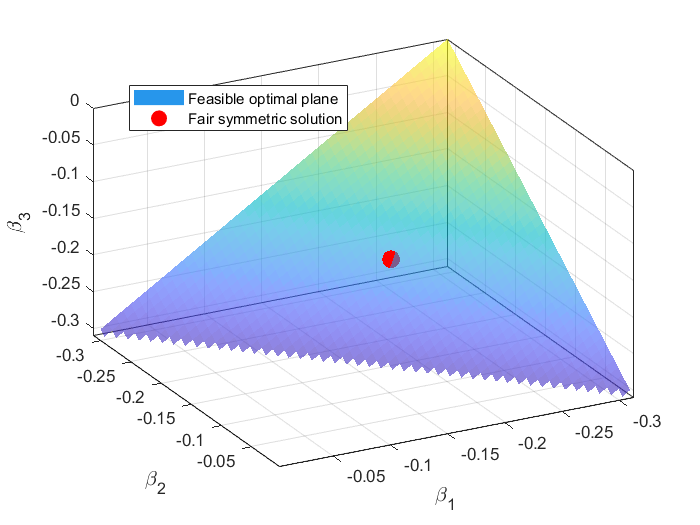
\includegraphics[width=1\linewidth]{figures/risk_seek_sol.png}
    \caption{Optimal $\beta_i$ Risk Seeking Solutions}
    \label{fig:beta_rs}
\end{figure}

Table~\ref{tab:comparison} and Figure~\ref{fig:algo1_comp_bars} summarize the performance of all four strategies. The risk-neutral Nash equilibrium incurs an $11.25\%$ profit loss relative to the coalition, while the risk-seeking Pareto-optimal Nash equilibrium fully recovers the coalition-level profit through risk coordination alone, without any change in the game structure. The distributed Algorithm~1 exactly reproduces the centralized Pareto-optimal result: each operator independently estimates $\hat{n}_i=3$ and $\hat{x}_r^o=300$\,MW from the consensus protocols, computes $\beta_i'=-\frac{1}{6}$, and submits the same bids and achieves the same profit as the centralized symmetric Pareto case.

\begin{table}[hbt!]
\centering
\caption{Performance Comparison of Bidding Strategies ($n=3$)}
\label{tab:comparison}
\begin{tabular}{lcccc}
\hline
Strategy & $\boldsymbol{\alpha}^*$ & $f$ & $g$\,(MW$^2$) & $\Pi$\,(\$/hr) \\
\hline
Coalition & $(0.50,\;0.50,\;0.50)$ & $0.50$ & 22{,}500 & 10{,}800 \\
RN Nash             & $(0.63,\;0.75,\;0.94)$ & $0.75$ & 16{,}875 &  9{,}675 \\
RS Pareto Nash      & $(0.42,\;0.50,\;0.63)$ & $0.50$ & 22{,}500 & 10{,}800 \\
Algo.~1 (Dist.)     & $(0.42,\;0.50,\;0.63)$ & $0.50$ & 22{,}500 & 10{,}800 \\
\hline
\end{tabular}
\end{table}

\begin{figure}[hbt!]
    \centering
    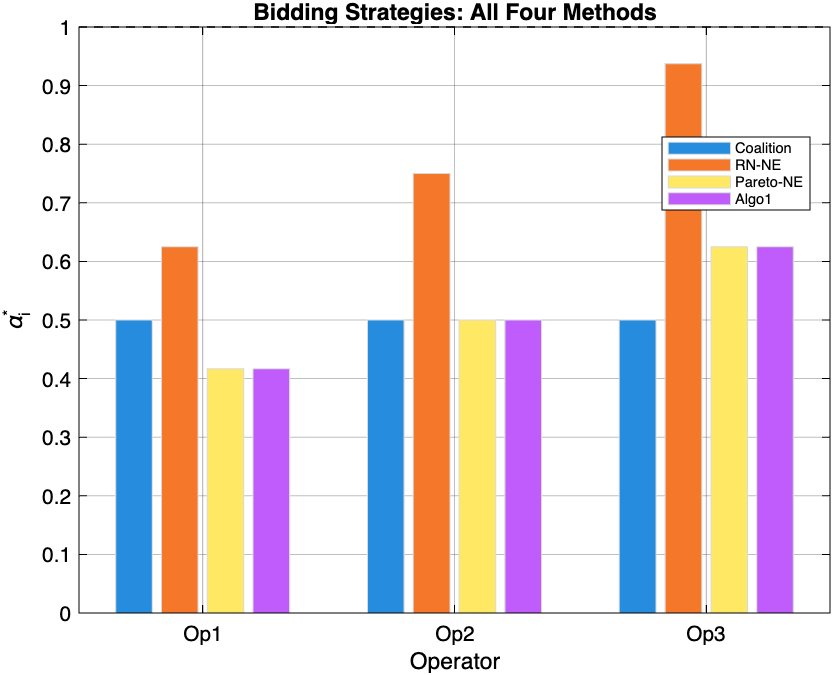
\includegraphics[width=0.48\linewidth]{figures/algorithm1_comp_alpha.png}%
    \hfill%
    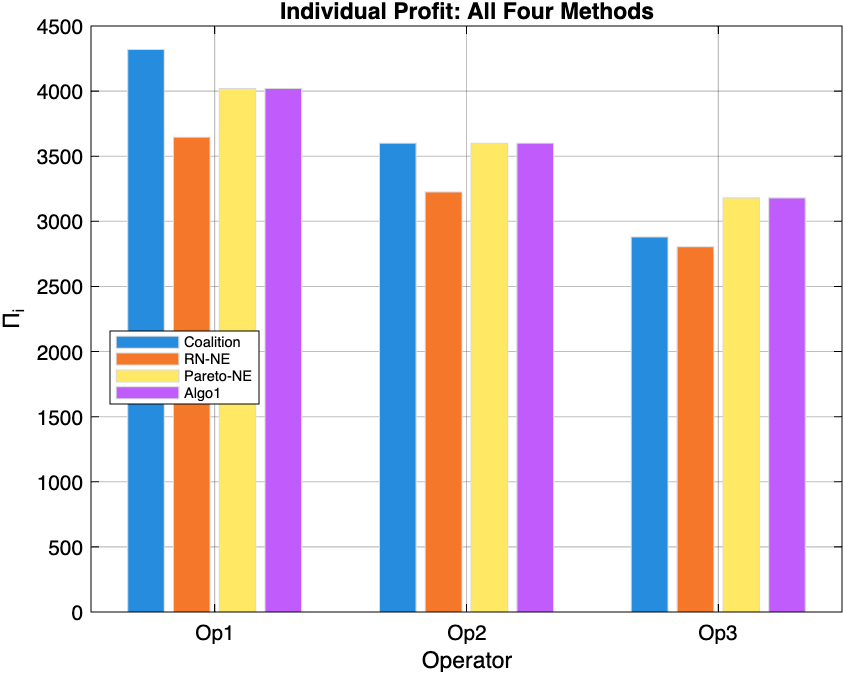
\includegraphics[width=0.48\linewidth]{figures/algorithm1_comp_profit.png}
    \caption{Bidding strategies $\alpha_i^*$ (left) and individual profits $\Pi_i$ (right) for all four strategies.}
    \label{fig:algo1_comp_bars}
\end{figure}

\subsection{Overbidding Analysis}

As established analytically, overbidding occurs for operator~$i$ whenever $\beta_i' > \frac{2\eta_i-1}{4}$ (bound~\eqref{eq:overbid_bound}), and the no-overbidding projection~\eqref{eq:alpha_clamp} incurs a profit loss~\eqref{eq:Pi_clamp}. Since the stochastic terms are constant offsets that do not affect the strategic comparison, the individual profit~\eqref{eq:Pi_j_exp} reduces to
\begin{equation}
\Pi_i(\boldsymbol{\alpha}) = 2a_2\,\alpha_i x_i^o x_r^o\bigl(1 - f(\boldsymbol{\alpha})\bigr) + a_1 x_i^o + 2a_2 x_i^o(x_L^o - x_r^o).
\label{eq:Pi_det}
\end{equation}
Define the saturation count as the number of operators whose unconstrained bids exceed capacity:
\begin{equation}
N_{\mathrm{sat}} = \sum_{i=1}^n \mathbf{1}\{\alpha_i^* > 1\}.
\label{eq:nsat}
\end{equation}
We sweep the common risk level $\beta' \in [-0.24,0.35]$, applying the projection~\eqref{eq:alpha_clamp} when needed, and for each $\beta'$ compare the aggregate payoff $\sum_i\Pi_i(\boldsymbol{\alpha})$ against $\sum_i\Pi_i(\bar{\boldsymbol{\alpha}})$ under the no-overbidding policy.

\begin{figure}[hbt!]
    \centering
    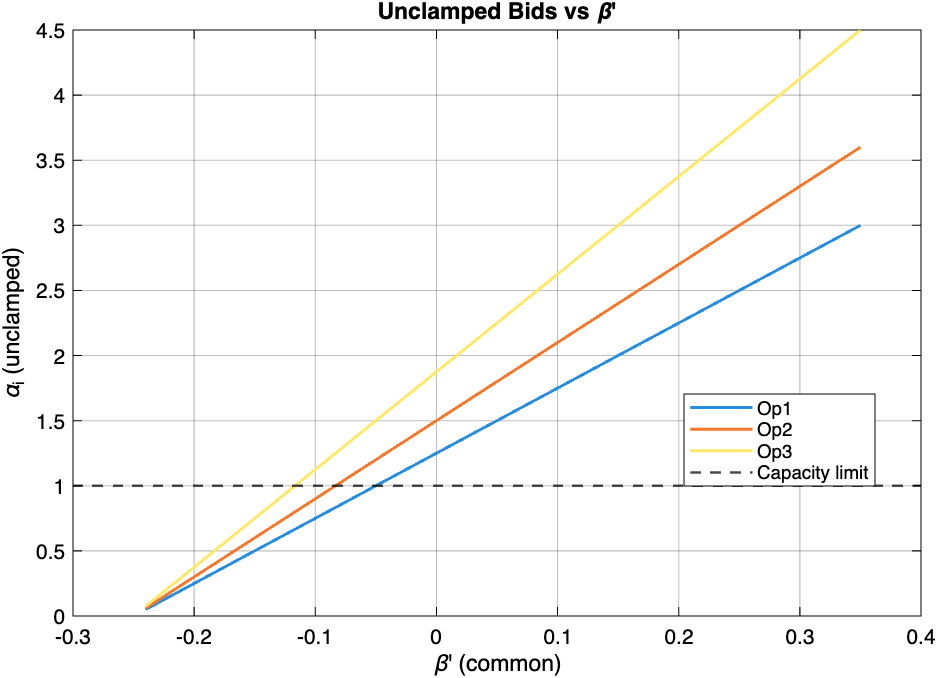
\includegraphics[width=1\linewidth]{figures/algorithm1_overbid_alpha.png}
    \caption{Unclamped bid levels versus common $\beta'$.}
    \label{fig:algo1_overbid_alpha}
\end{figure}

\begin{figure}[hbt!]
    \centering
    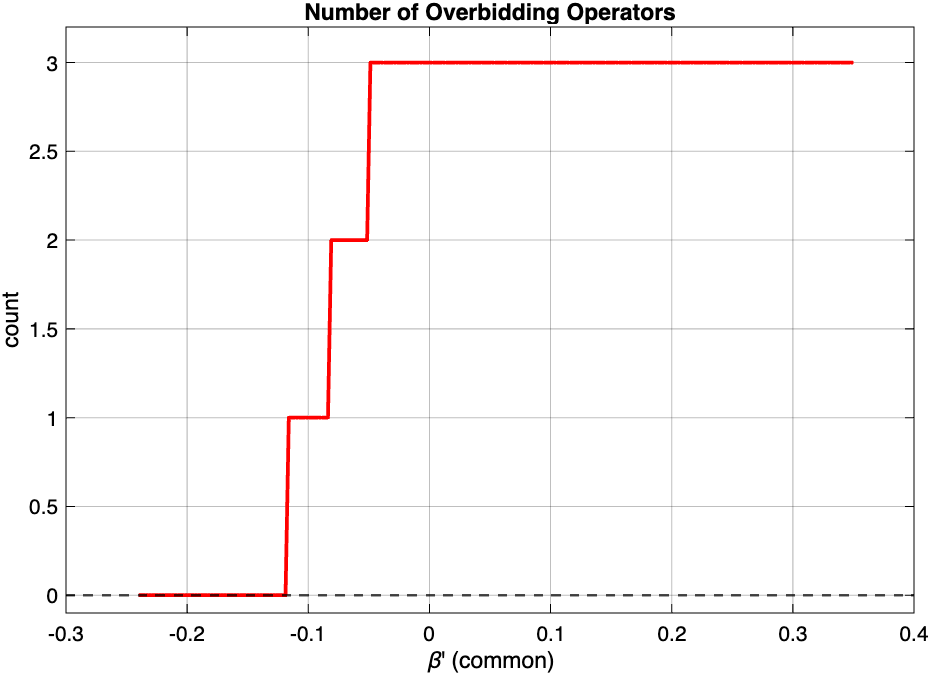
\includegraphics[width=1\linewidth]{figures/algorithm1_overbid_count.png}
    \caption{Number of operators with $\alpha_i>1$ versus $\beta'$.}
    \label{fig:algo1_overbid_count}
\end{figure}

\begin{figure}[hbt!]
    \centering
    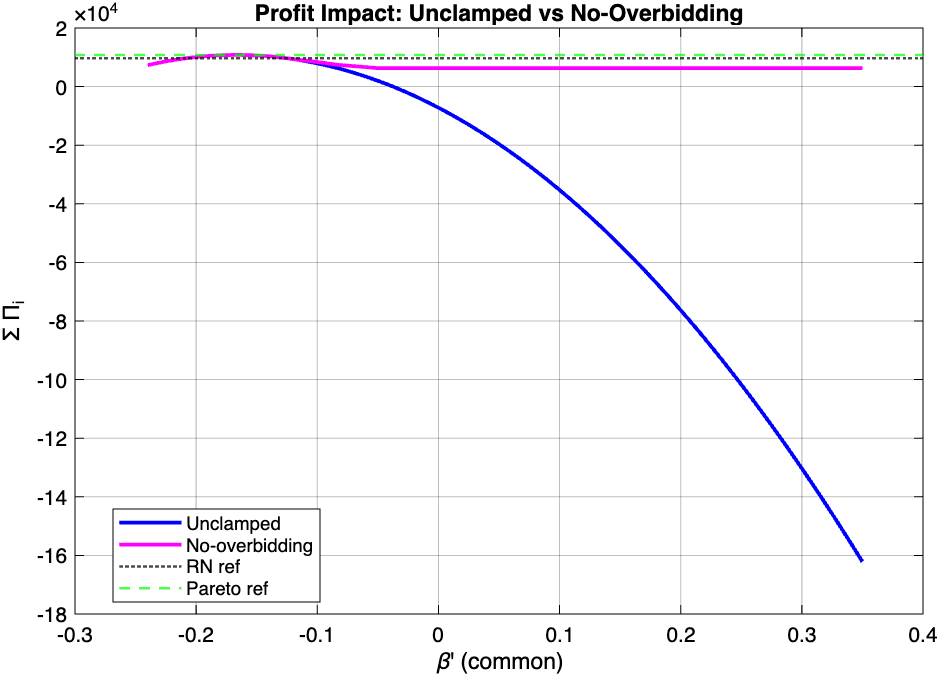
\includegraphics[width=1\linewidth]{figures/algorithm1_overbid_profit.png}
    \caption{Aggregate profit comparison: unconstrained versus no-overbidding projection.}
    \label{fig:algo1_overbid_profit}
\end{figure}

\begin{figure}[hbt!]
    \centering
    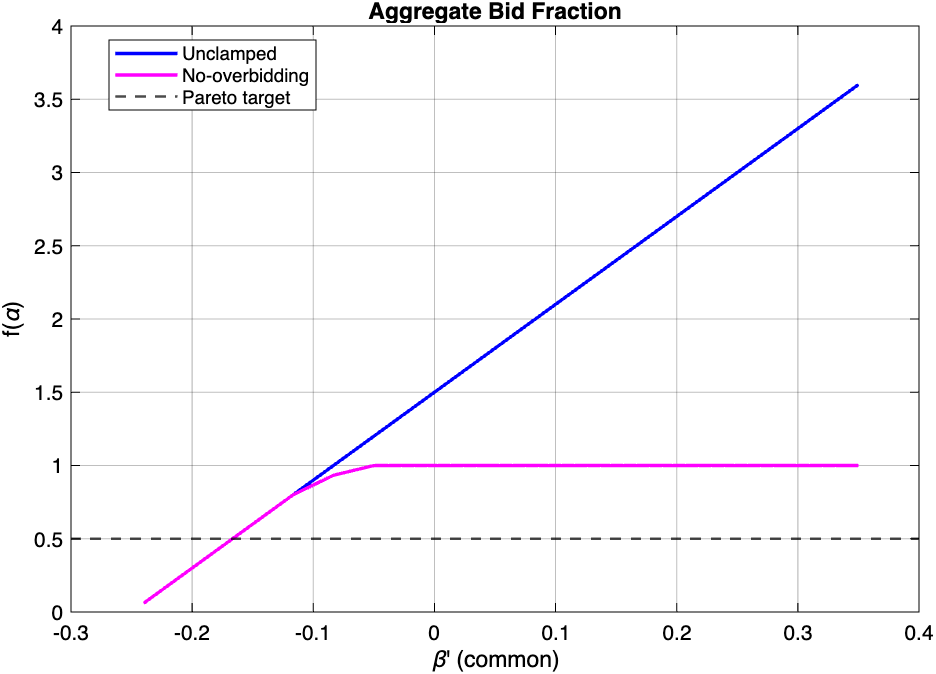
\includegraphics[width=1\linewidth]{figures/algorithm1_overbid_f.png}
    \caption{Aggregate bid fraction $f(\boldsymbol{\alpha})$ under unconstrained and no-overbidding models.}
    \label{fig:algo1_overbid_f}
\end{figure}

Figures~\ref{fig:algo1_overbid_alpha}--\ref{fig:algo1_overbid_f} quantify the tradeoff introduced by overbidding. For fixed $\beta'$, smaller $\eta_i$ yields larger unconstrained bids~\eqref{eq:alpha_optimal_simplified}, so operators with lower renewable share saturate first as $\beta'$ increases. The projection~\eqref{eq:alpha_clamp} shifts $f(\boldsymbol{\alpha})$ away from $\frac{1}{2}$ and thereby reduces both $g(\boldsymbol{\alpha})$ and $\sum_i\Pi_i$ through~\eqref{eq:Pi_det}, explaining why the clamped and unclamped trajectories diverge under the same risk-parameter sweep.

\noindent\textbf{Remark~1.} \textit{For the three-operator system in Table~\ref{tab:example_params}, the capacity shares $\eta_1=\frac{2}{5}$, $\eta_2=\frac{1}{3}$, $\eta_3=\frac{4}{15}$ give per-operator overbidding thresholds $\beta_1'\leq-\frac{1}{20}=-0.05$, $\beta_2'\leq-\frac{1}{12}\approx-0.083$, $\beta_3'\leq-\frac{7}{60}\approx-0.117$ from~\eqref{eq:overbid_bound}. Under a common $\beta'$, operator~3 (smallest share) saturates first at $\beta'>-0.117$, followed by operator~2 at $\beta'>-0.083$ and operator~1 at $\beta'>-0.05$; the count~\eqref{eq:nsat} steps from $N_{\mathrm{sat}}=0$ to $3$ accordingly. The symmetric Pareto allocation $\beta_i'=-\frac{1}{6}\approx-0.167$ lies below all thresholds, so no overbidding occurs at the Pareto-optimal Nash equilibrium. Profit loss grows appreciably only once $N_{\mathrm{sat}}\geq 2$, with the aggregate trajectory diverging sharply from the unconstrained case beyond $\beta'>-0.083$.}

\subsection{Solutions under Distributed Algorithms}

Figures~\ref{fig:algo1_xi}--\ref{fig:algo1_psi} show convergence of the consensus states. The initial conditions follow Algorithm~\ref{alg:dist_risk_aware}: the utility sets $\xi_4(0)=1$, $\psi_4(0)=0$; each operator sets $\xi_i(0)=0$, $\psi_i(0)=x_i^o$. All agents converge to the common average $\xi_i(k)\to\frac{1}{4}$ and $\psi_i(k)\to\frac{x_r^o}{4}=75$\,MW. From these converged values, each operator~$i$ locally computes the quantities shown in Table~\ref{tab:algo1_computed}, confirming that every operator independently recovers the correct $\hat{n}_i=3$, $\eta_i$, and $\beta_i'=-\frac{1}{6}$ without any additional communication.

\begin{figure}[hbt!]
    \centering
    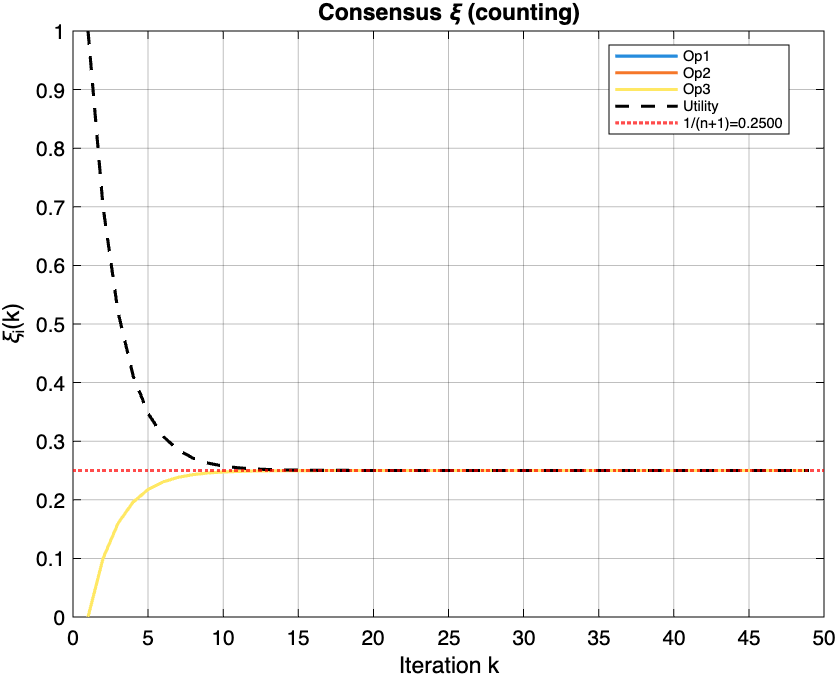
\includegraphics[width=1\linewidth]{figures/algorithm1_xi_consensus.png}
    \caption{Algorithm~1 consensus trajectory for $\xi_i$ (converges to $1/(n+1)=0.25$).}
    \label{fig:algo1_xi}
\end{figure}

\begin{figure}[hbt!]
    \centering
    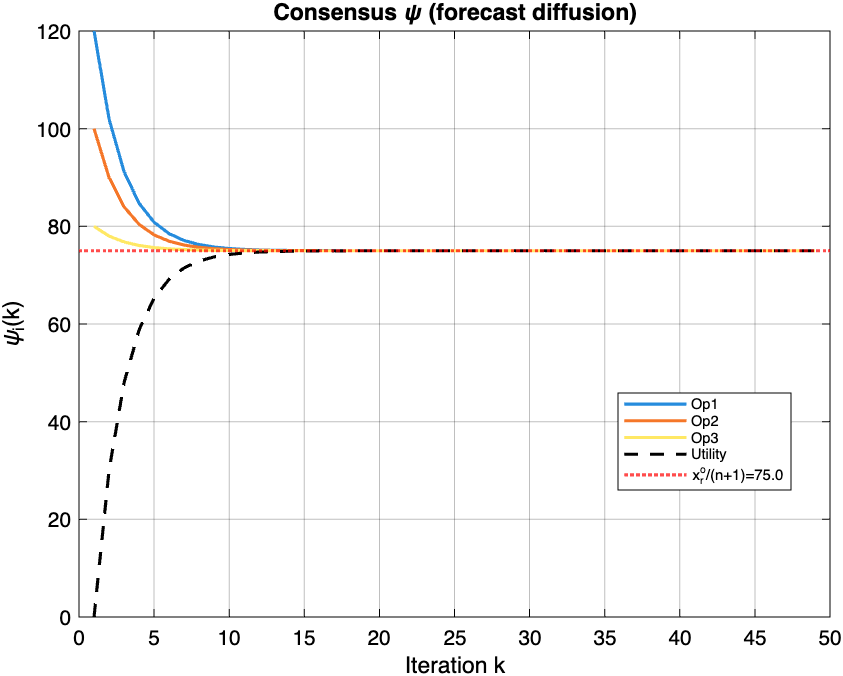
\includegraphics[width=1\linewidth]{figures/algorithm1_psi_consensus.png}
    \caption{Algorithm~1 consensus trajectory for $\psi_i$ (converges to $x_r^o/(n+1)=75$\,MW).}
    \label{fig:algo1_psi}
\end{figure}

\begin{table}[hbt!]
\centering
\caption{Quantities computed locally by each operator after consensus convergence}
\label{tab:algo1_computed}
\begin{tabular}{lcccc}
\hline
Op. & $\xi_i^\infty$ & $\hat{n}_i = 1/\xi_i^\infty - 1$ & $\eta_i = x_i^o\xi_i^\infty/\psi_i^\infty$ & $\beta_i' = (1-\hat{n}_i)/(4\hat{n}_i)$ \\
\hline
1 & 0.25 & 3 & $2/5$ & $-1/6\approx-0.167$ \\
2 & 0.25 & 3 & $1/3$ & $-1/6\approx-0.167$ \\
3 & 0.25 & 3 & $4/15$ & $-1/6\approx-0.167$ \\
\hline
\end{tabular}
\end{table}
\begin{figure}[hbt!]
    \centering
    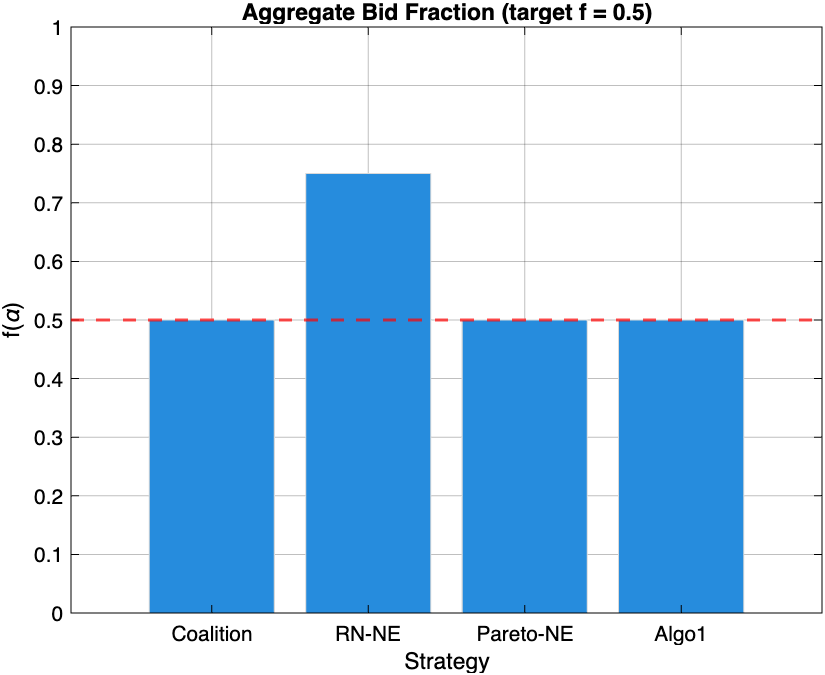
\includegraphics[width=0.48\linewidth]{figures/algorithm1_comp_f.png}%
    \hfill%
    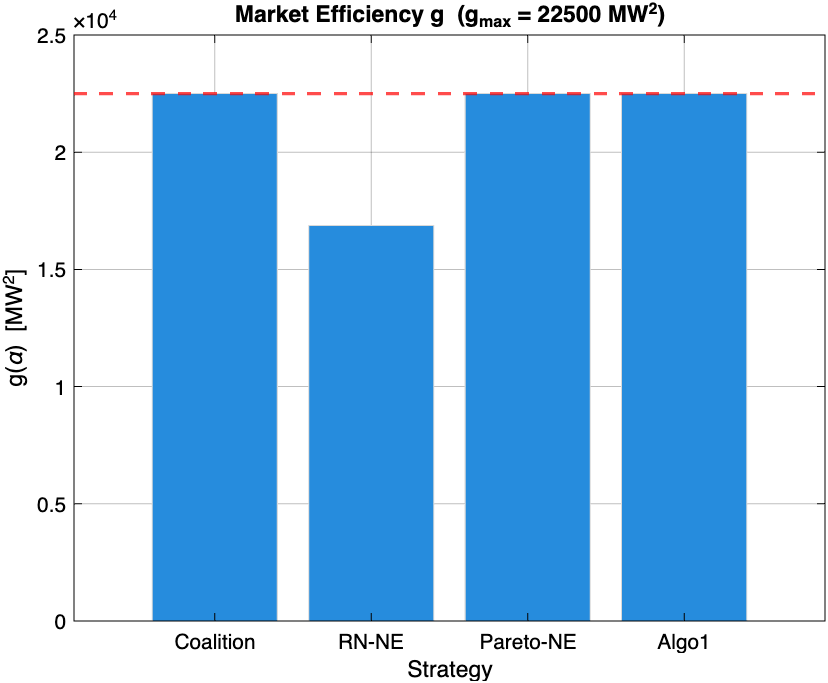
\includegraphics[width=0.48\linewidth]{figures/algorithm1_comp_g.png}
    \caption{Aggregate bid fraction $f(\boldsymbol{\alpha})$ (left, target $f=0.5$ dashed) and market efficiency $g(\boldsymbol{\alpha})$ (right, $g_{\max}$ dashed) for all four strategies.}
    \label{fig:algo1_comp_fg}
\end{figure}


\begin{comment}
    

\subsubsection{Algorithm 2: Non-Equal Initial Risk Parameters}
Algorithm~\ref{alg:dist_risk_aware_beta_coord} is evaluated using \texttt{risk\_aware\_power\_system.m} under multiple heterogeneous initial conditions $\beta_i'(0)$. The study focuses on whether distributed coordination of the aggregate risk parameter and unclamped one-shot bidding preserve the Pareto target. Accordingly, bid/profit comparisons are reported in this subsection (after the risk-parameter coordination stage is complete).

\begin{figure}[hbt!]
    \centering
    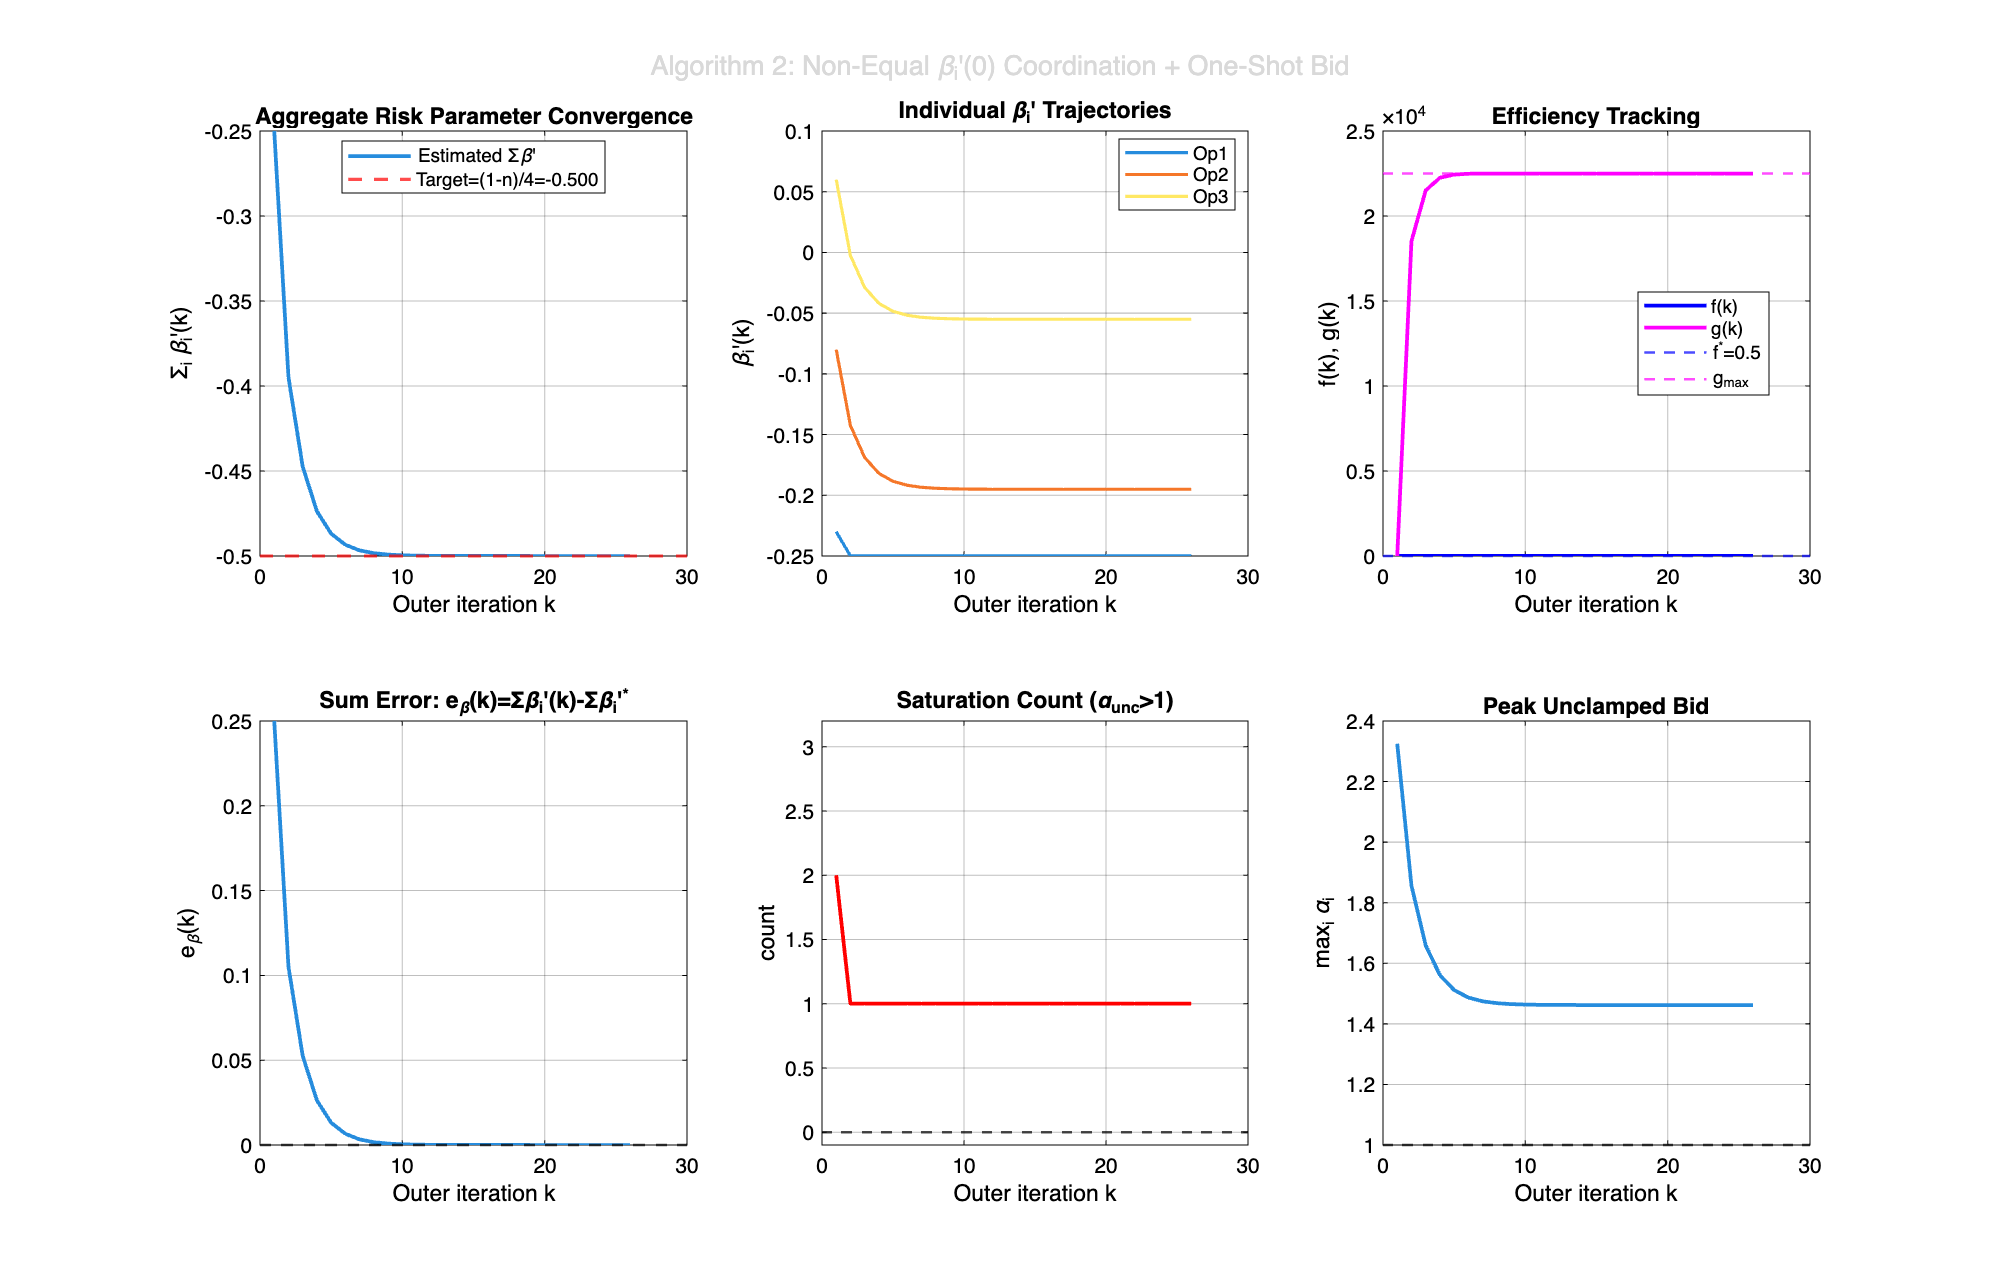
\includegraphics[width=1\linewidth]{figures/algorithm2_results.png}
    \caption{Algorithm~2 single-scenario diagnostics: convergence of $\sum\beta_i'$, individual $\beta_i'$, efficiency metrics, and saturation count.}
    \label{fig:algo2_single}
\end{figure}

\begin{figure}[hbt!]
    \centering
    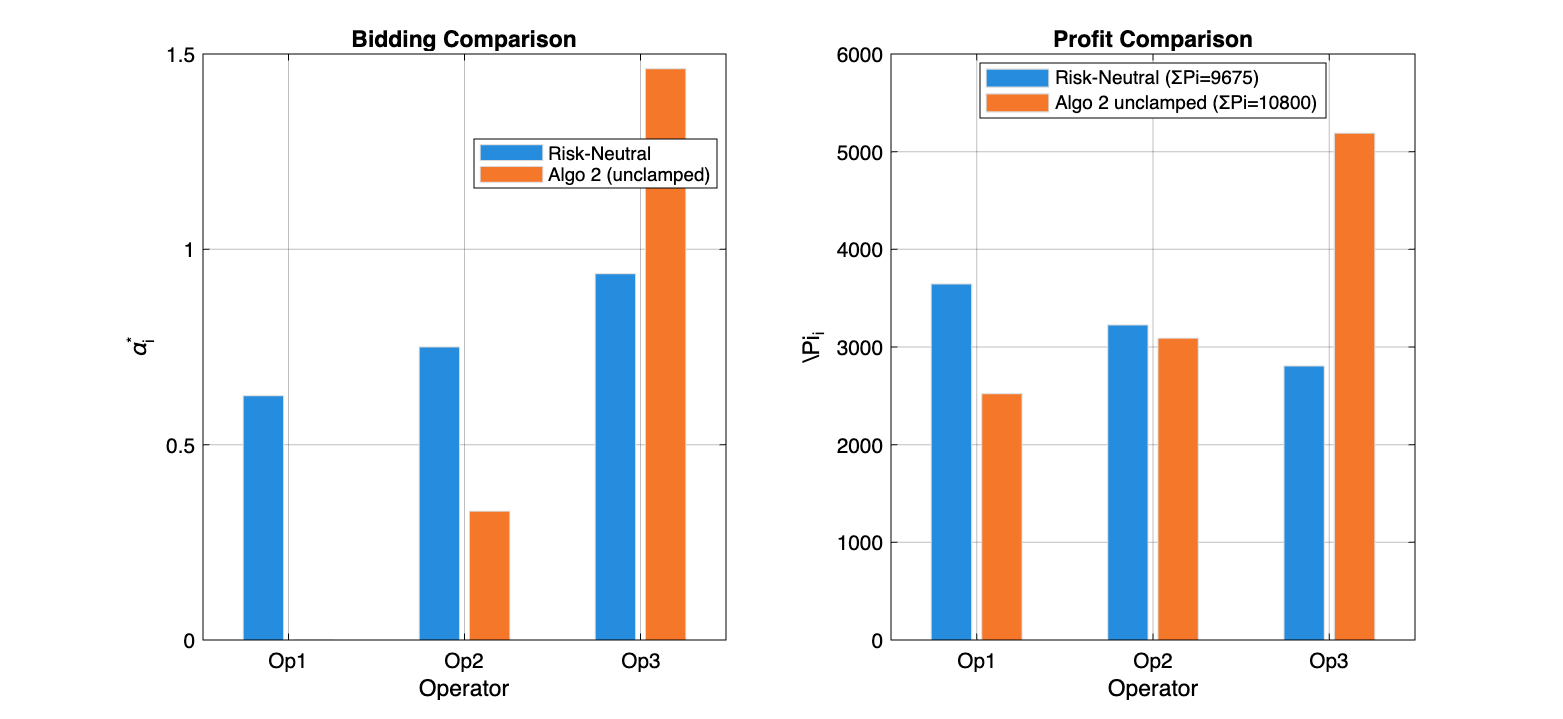
\includegraphics[width=1\linewidth]{figures/algorithm2_bidding_comparison.png}
    \caption{Algorithm~2 bidding/profit comparison under the unclamped $\alpha_i$ assumption.}
    \label{fig:algo2_bidprofit}
\end{figure}

\begin{figure}[hbt!]
    \centering
    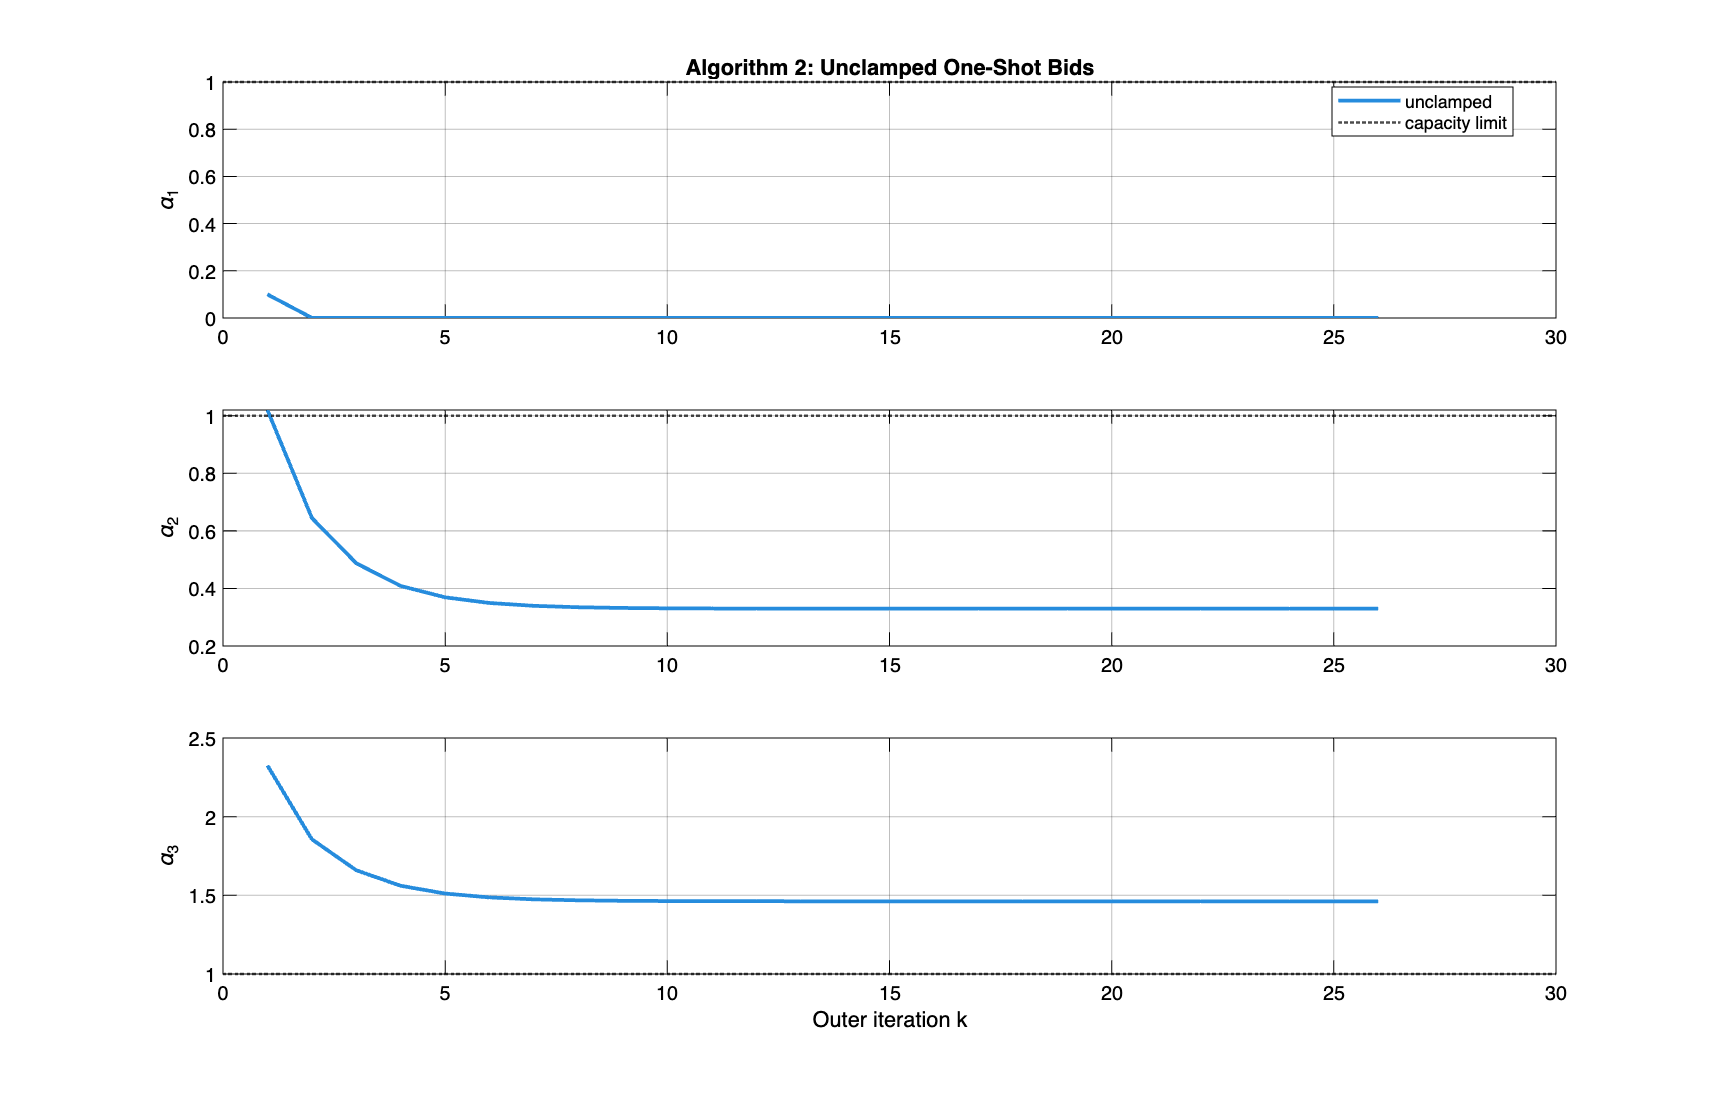
\includegraphics[width=1\linewidth]{figures/algorithm2_alpha_unclamped.png}
    \caption{Algorithm~2 one-shot bid trajectories under the unclamped $\alpha_i$ assumption, with capacity limit shown for reference.}
    \label{fig:algo2_clamp}
\end{figure}

\begin{table}[h]
\centering
\caption{Test cases with initial transformed risk parameters $\beta_i' = a_2\beta_i$}
\label{tab:test_cases}
\begin{tabular}{lcccc}
\hline
Test case & $\beta_1'$ & $\beta_2'$ & $\beta_3'$ & Risk Profile \\
\hline
I & 0 & 0 & 0 & Risk-neutral \\
II & -1 & -1 & -1 & Risk-seeking \\
III & 1 & 1 & 1 & Risk-averse \\
IV & -1 & 1 & 1 & Mixed \\
V & -0.25 & 0 & 0.20 & Mixed \\
VI & -0.25 & 0 & 0 & Mixed \\
\hline
\end{tabular}
\end{table}

\begin{figure}[hbt!]
    \centering
    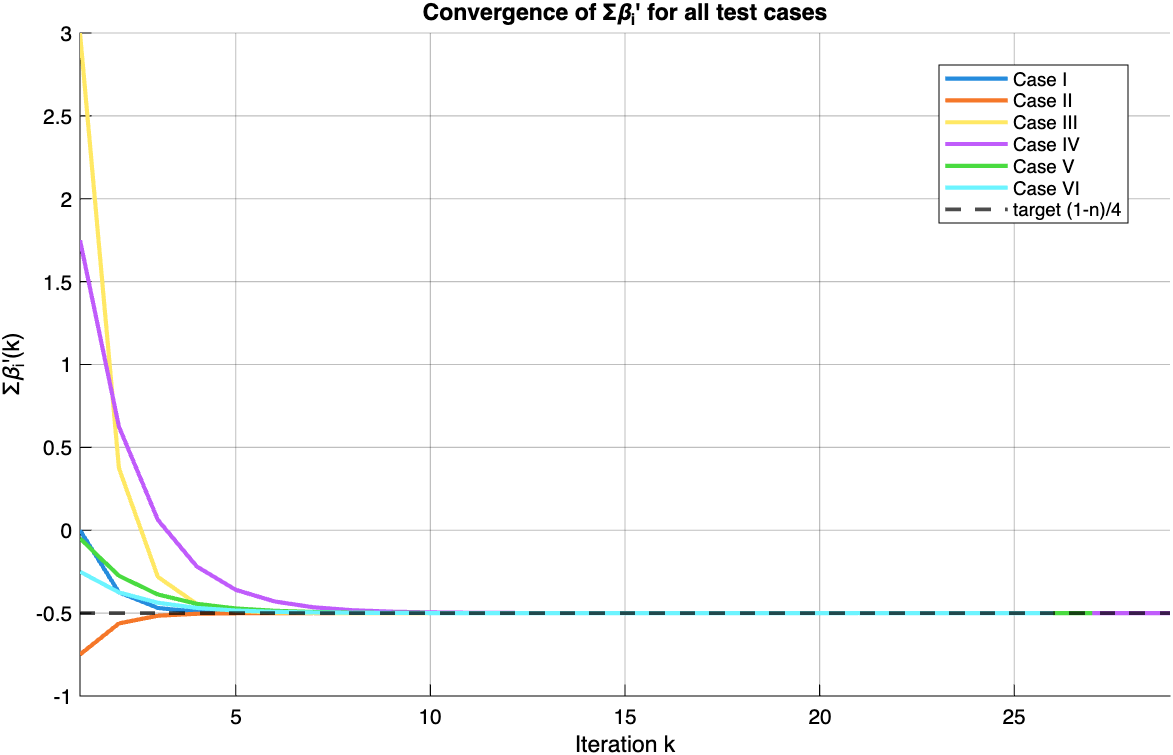
\includegraphics[width=1\linewidth]{figures/sum_beta_convergence_all_cases.png}
    \caption{Convergence of $\sum\beta_i'$ for all test cases. Each case converges to the Pareto-optimal sum $\sum\beta_i'^* = (1-n)/4 = -0.5$.}
    \label{fig:sum_beta_all}
\end{figure}

\begin{figure}[hbt!]
    \centering
    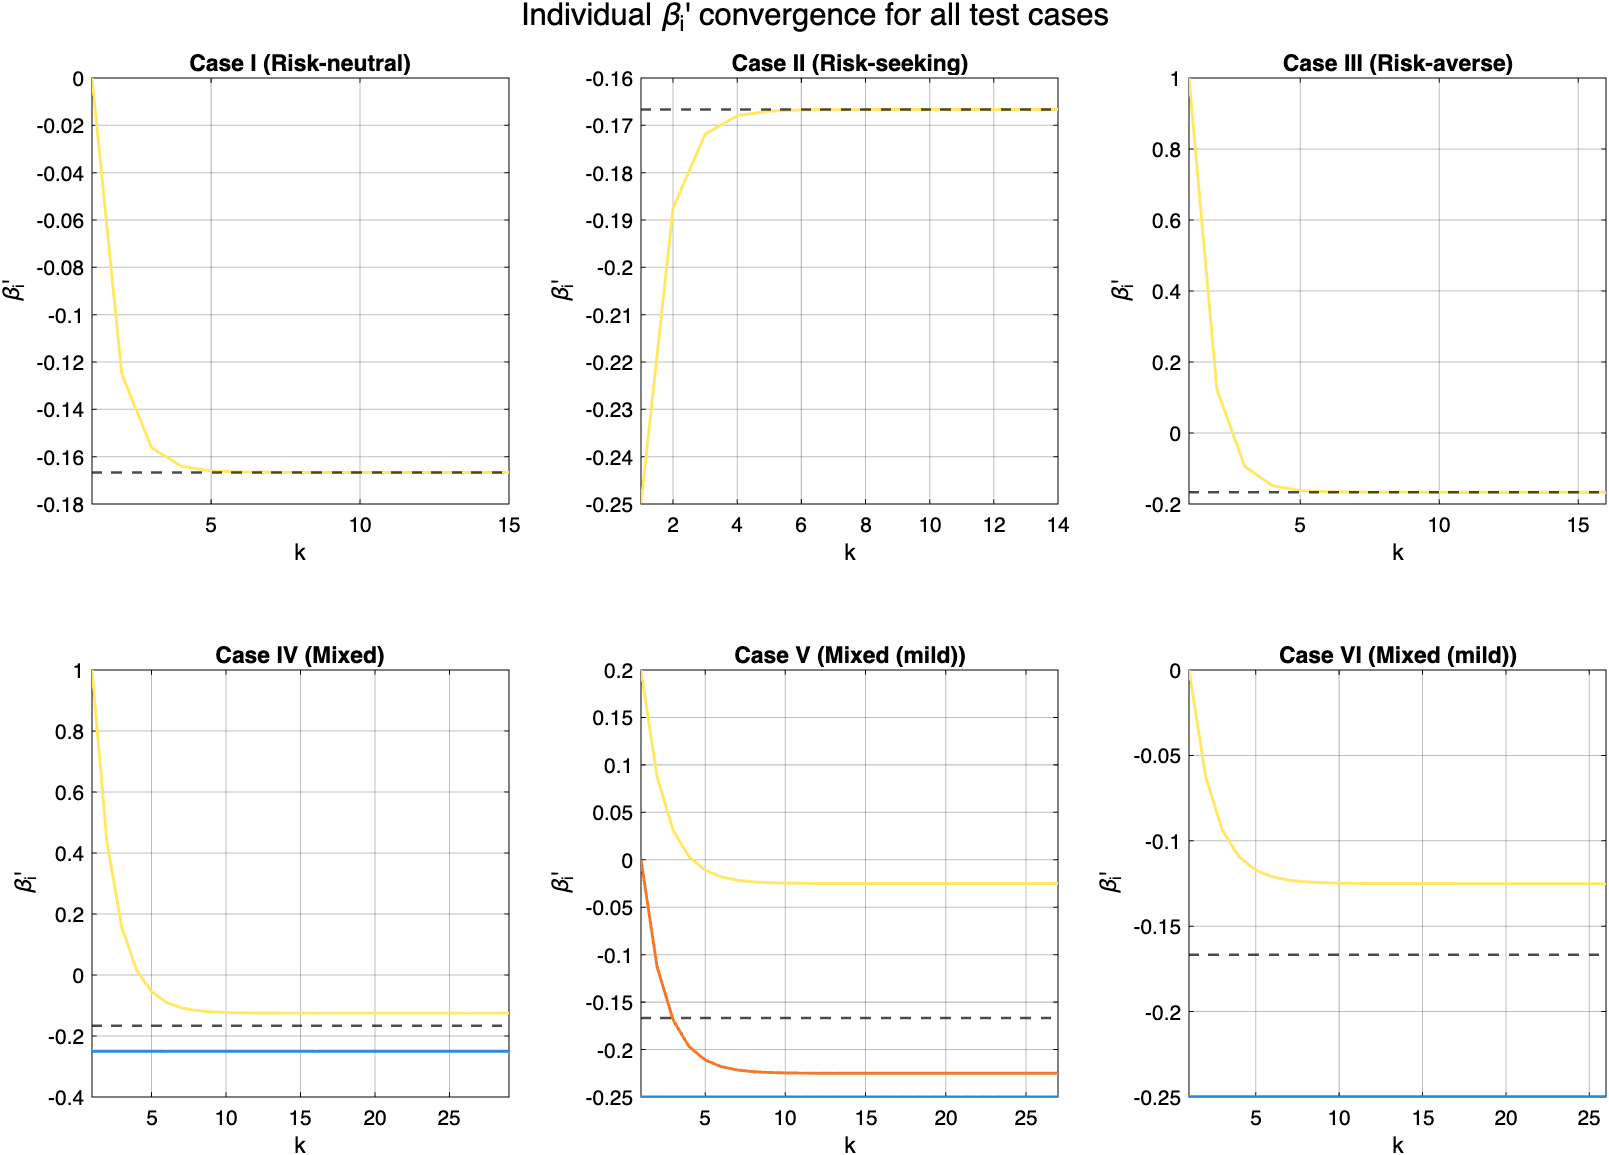
\includegraphics[width=1\linewidth]{figures/beta_individual_all_cases.png}
    \caption{Individual $\beta_i'$ convergence for each test case. Most cases achieve the Pareto-optimal sum; cases with capacity-constrained operators may converge to alternative equilibria (see Remark~1).}
    \label{fig:beta_individual}
\end{figure}

\begin{figure}[hbt!]
    \centering
    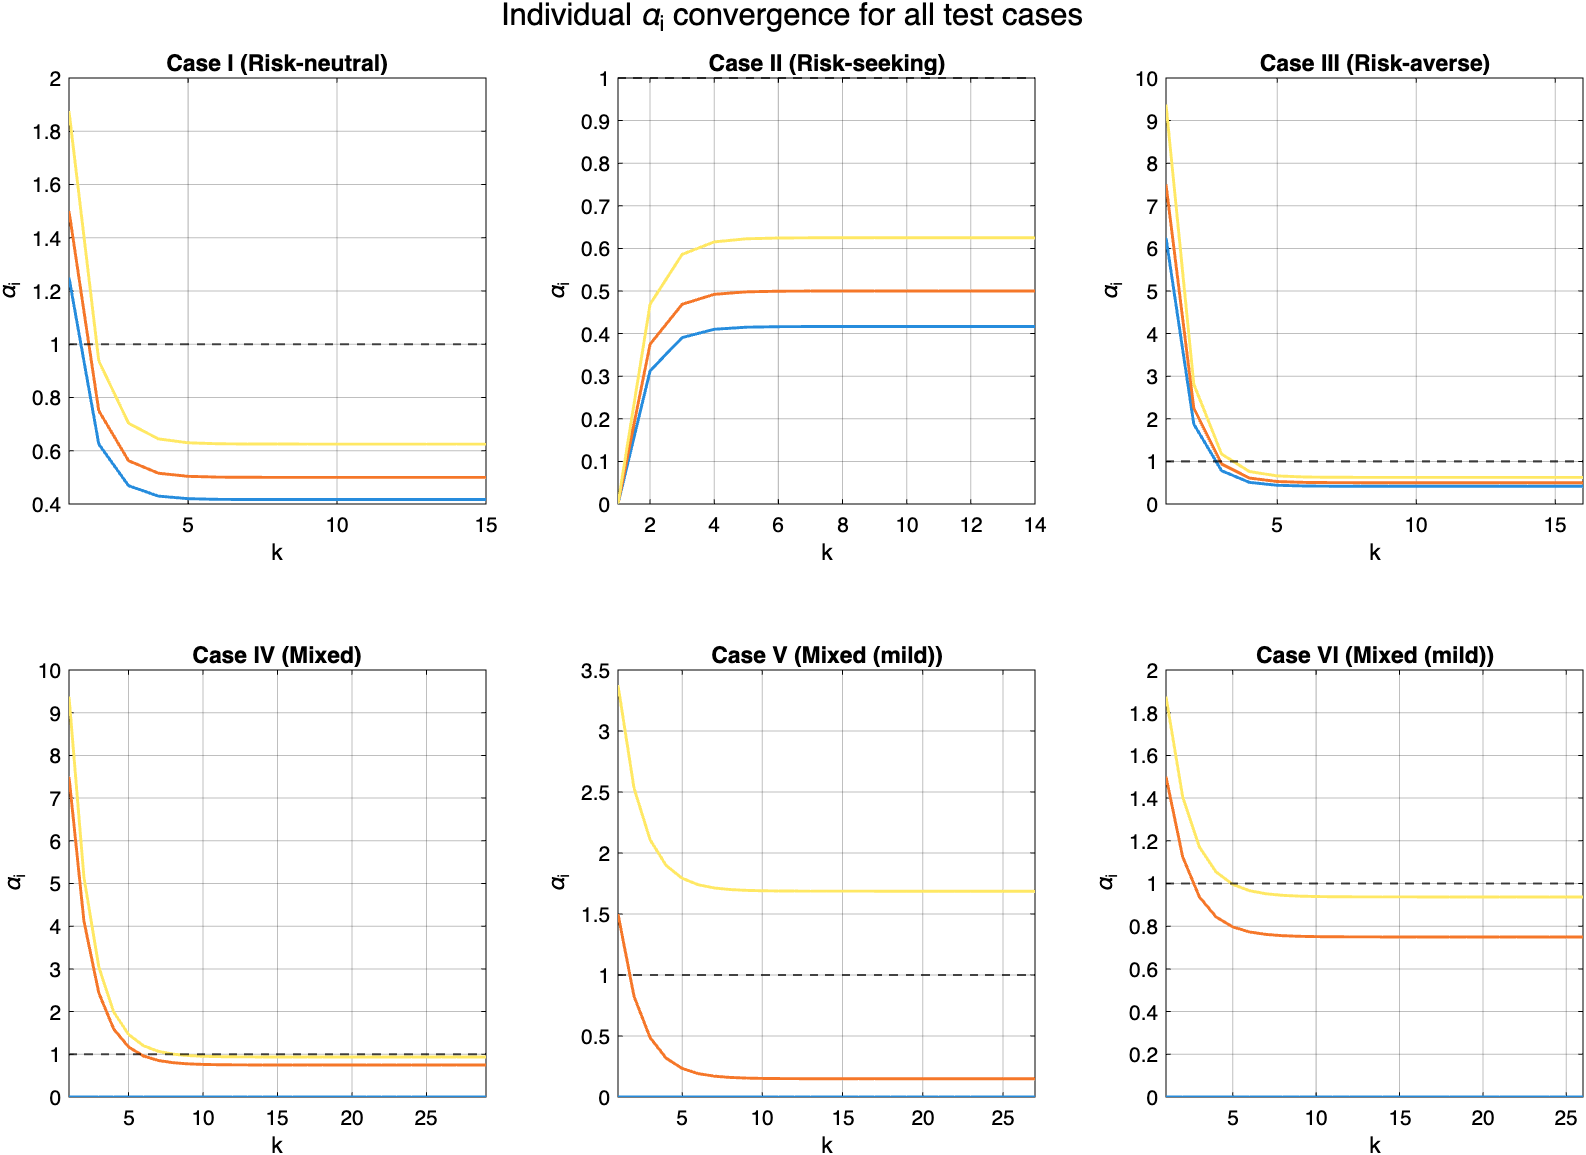
\includegraphics[width=1\linewidth]{figures/alpha_individual_all_cases.png}
    \caption{Individual $\alpha_i$ convergence for each test case. Bidding fractions adjust to achieve $f(\alpha) = 0.5$.}
    \label{fig:alpha_individual}
\end{figure}

Figure~\ref{fig:sum_beta_all} shows the convergence of the aggregate risk parameter $\sum\beta_i'$ for all test cases. Despite vastly different initial conditions ranging from risk-neutral (Case~I) to risk-seeking (Case~II) to risk-averse (Case~III) to mixed profiles (Cases~IV--VI), most cases converge to the Pareto-optimal value $\sum\beta_i'^* = (1-n)/4 = -0.5$ as predicted by Theorem~2. For cases with highly asymmetric initial risk preferences where capacity constraints bind (see Remark~1), the algorithm may converge to a different $\sum\beta_i'$ while still driving $f(\alpha)$ close to $0.5$ under the unclamped-bid model. Figure~\ref{fig:beta_individual} provides a detailed view of individual $\beta_i'$ trajectories within each case, showing how operators with different initial risk preferences adapt their parameters.

Figure~\ref{fig:alpha_individual} shows the corresponding evolution of bidding fractions $\alpha_i$. As the risk parameters converge, the bidding strategies adjust to achieve $f(\alpha) = 0.5$, confirming the Nash equilibrium behavior characterized in Lemma~2. Figures~\ref{fig:algo2_single}, \ref{fig:algo2_bidprofit}, and~\ref{fig:algo2_clamp} further illustrate the single-scenario dynamics of Algorithm~2 under the unclamped-bid assumption. The impact of the risk-parameter updates on market efficiency is illustrated in Figures~\ref{fig:f_all} and~\ref{fig:S_all}, where the aggregate bidding fraction $f(\alpha)$ converges to $1/2$ and the error signal $|S|$ decreases below the convergence tolerance for all test cases.

\begin{figure}[hbt!]
    \centering
    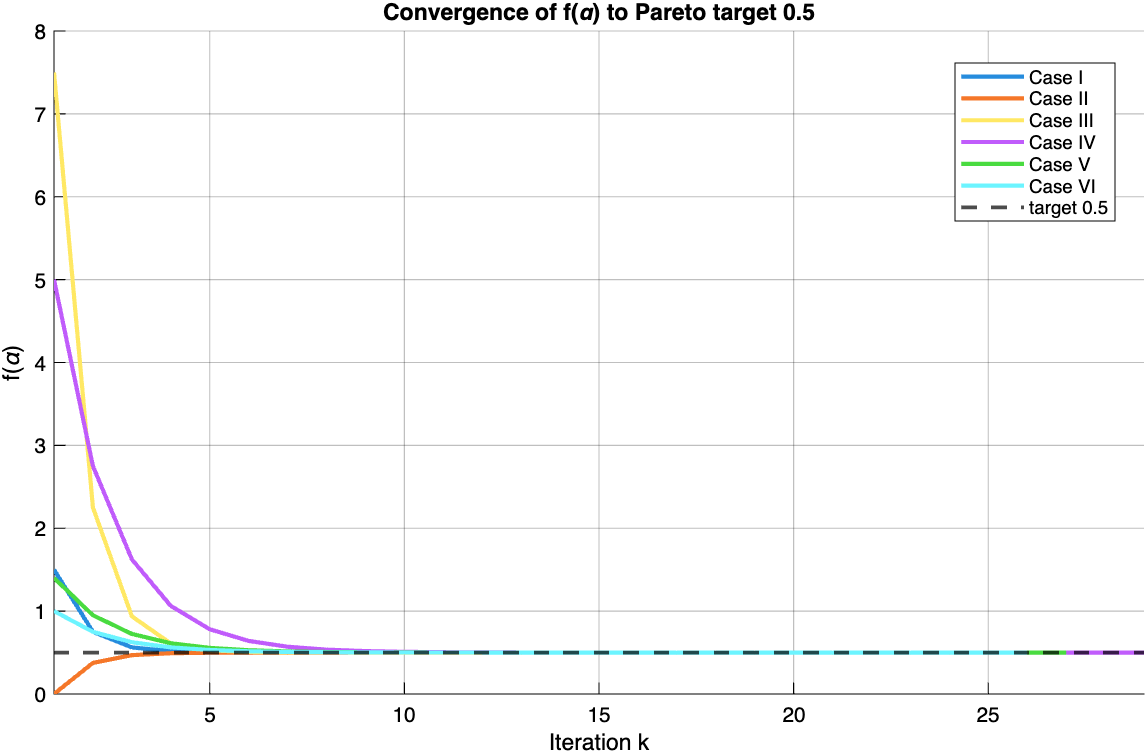
\includegraphics[width=1\linewidth]{figures/f_convergence_all_cases.png}
    \caption{Convergence of aggregate bidding fraction $f(\alpha)$ to Pareto target $0.5$ for all test cases.}
    \label{fig:f_all}
\end{figure}

\begin{figure}[hbt!]
    \centering
    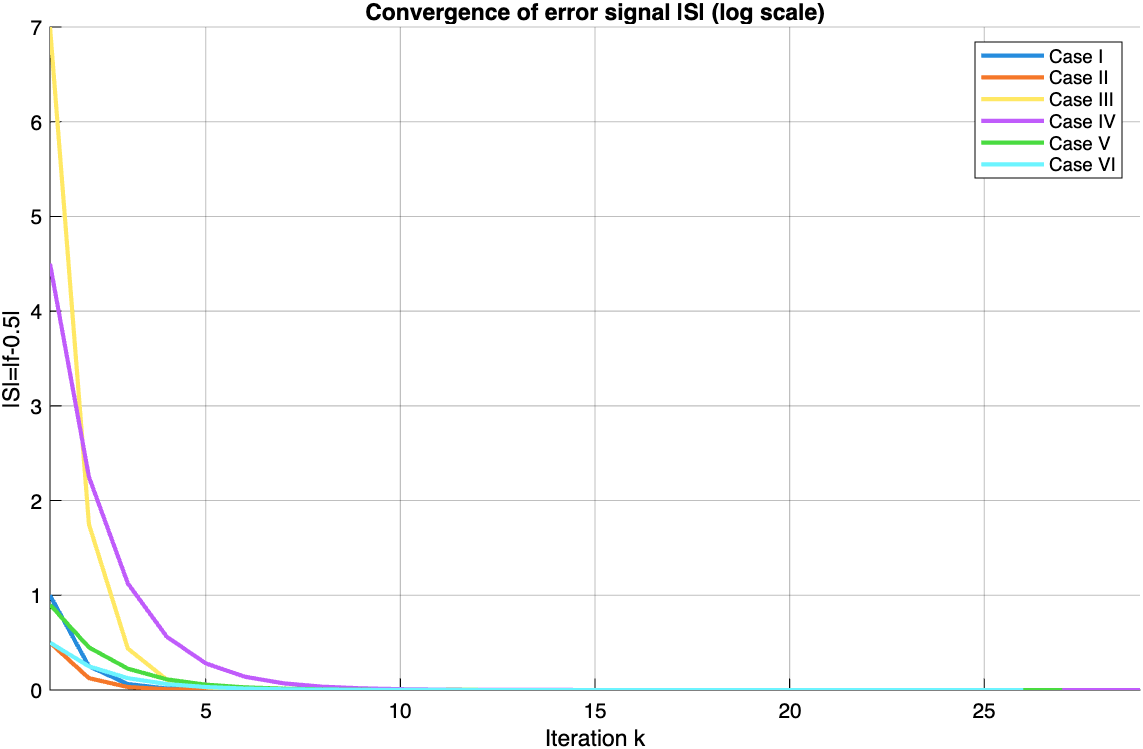
\includegraphics[width=1\linewidth]{figures/S_convergence_all_cases.png}
    \caption{Convergence of error signal $|S| = |f - 0.5|$ (log scale) for all test cases.}
    \label{fig:S_all}
\end{figure}

\begin{figure}[hbt!]
    \centering
    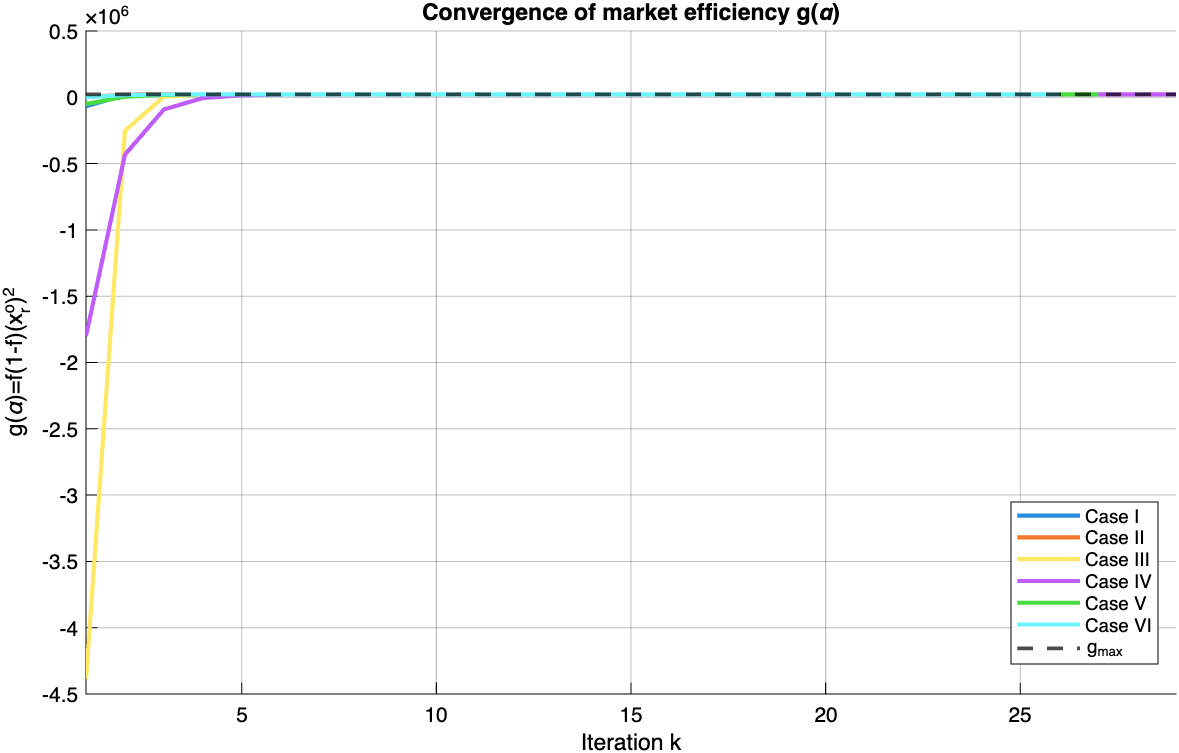
\includegraphics[width=1\linewidth]{figures/g_convergence_all_cases.png}
    \caption{Convergence of market efficiency $g(\alpha) = f(1-f)(x_r^o)^2$ to maximum value $g_{\max} = 0.25(x_r^o)^2$ for all test cases.}
    \label{fig:g_all}
\end{figure}

\begin{figure}[hbt!]
    \centering
    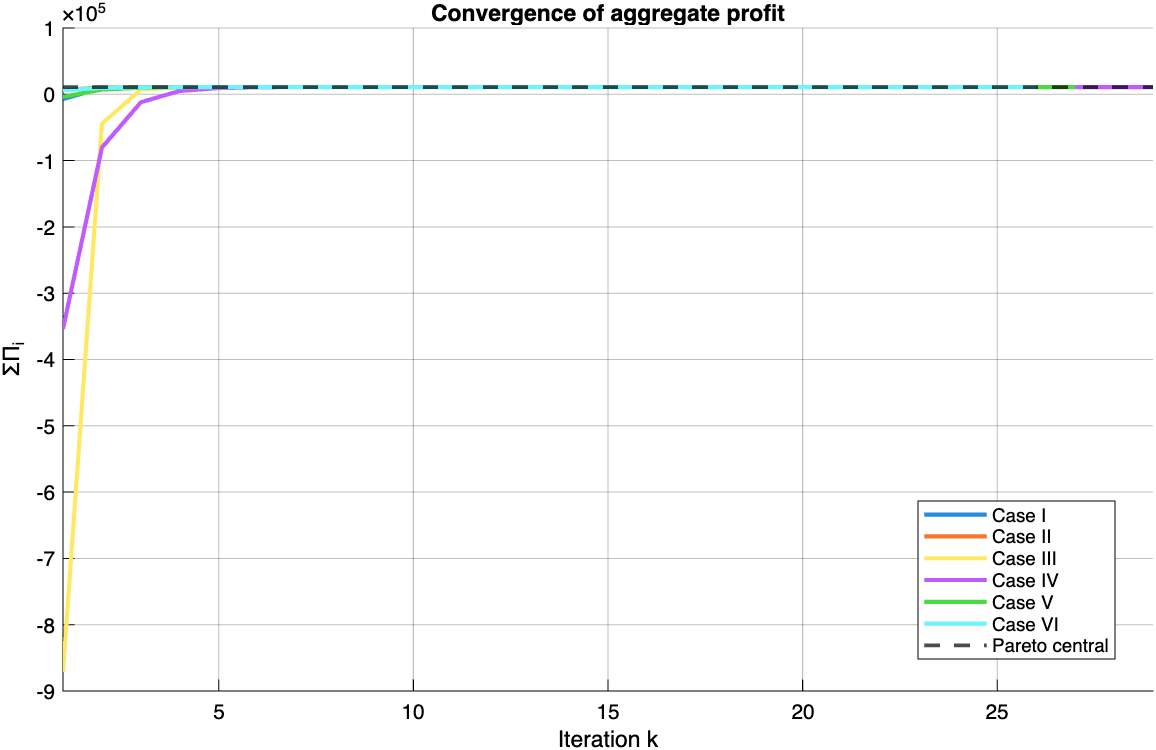
\includegraphics[width=1\linewidth]{figures/profit_convergence_all_cases.png}
    \caption{Convergence of aggregate profit $\sum\Pi_i$ for all test cases.}
    \label{fig:profit_all}
\end{figure}

Figure~\ref{fig:g_all} demonstrates that market efficiency $g(\alpha)$ converges to its maximum value $g_{\max} = 0.25(x_r^o)^2 = 22{,}500$ for all test cases, confirming that the distributed algorithm successfully achieves Pareto optimality. Figure~\ref{fig:profit_all} shows the corresponding convergence of aggregate profits $\sum\Pi_i$.

Notably, for mixed risk profiles where some operators are risk-seeking while others are risk-averse (e.g., Case~V), the unconstrained model can produce $\alpha_i>1$ for risk-averse operators, as discussed in Remark~1. In such cases, the aggregate risk parameter $\sum\beta_i'$ may not converge exactly to $(1-n)/4$; yet the algorithm still drives $f(\alpha)$ toward $0.5$ and near-Pareto aggregate profit. This demonstrates the robustness of the distributed approach under heterogeneous risk preferences.

These results validate that the proposed distributed algorithm achieves Pareto-enhanced Nash equilibria using only local computations and minimal information exchange. Regardless of initial risk preferences, the algorithm guides all operators toward the collective optimum. In particular, the renewable operators do not require knowledge of other agents' forecasts, cost parameters, or private objectives, yet collectively achieve the same performance as a centralized optimizer. This highlights the practicality of the proposed framework for real-time electricity markets with decentralized renewable participants.
\end{comment}

\section{Conclusion}

This paper presented a risk-aware bidding framework in which the risk sensitivity parameter $\beta_i$ acts as a coordination variable for renewable generation operators in electricity markets. We showed that the noncooperative game admits structured Nash equilibria and that, by appropriate risk allocation, these equilibria can recover Pareto-efficient aggregate outcomes. In particular, the analysis established explicit relationships between risk parameters, bidding coefficients, and market efficiency.

A distributed consensus-based implementation was developed for the one-shot strategy, allowing each operator to estimate required aggregate quantities using only local communication. The illustrative example confirmed that the distributed Algorithm~1 reproduces the targeted bidding behavior without centralized disclosure of private forecasts or cost data. Additional sensitivity analysis on overbidding showed how unconstrained bids can exceed physical limits and how no-overbidding projection changes aggregate bidding fraction and profit trajectories, directly quantifying the performance impact of feasibility constraints.

Overall, the results demonstrate that risk-aware design can align self-interested bidding with improved collective efficiency while preserving decentralization and privacy. Future work will incorporate network congestion and locational pricing, extend to 
non-Gaussian uncertainty structures and time-varying operator participation, and analyze robustness under communication delay, packet loss, and adversarial behavior.

\bibliographystyle{IEEEtran}
\bibliography{references}

\end{document}